% ------------------------------------------------------------
% LaTeX Template für die DHBW zum Schnellstart!
% Original: https://github.wdf.sap.corp/vtgermany/LaTeX-Template-DHBW
% ------------------------------------------------------------
% ---- Präambel mit Angaben zum Dokument
\documentclass[
	fontsize=12pt,           % Leitlinien sprechen von Schriftgröße 12.
	paper=A4,
	twoside=false,
	listof=totoc,            % Tabellen- und Abbildungsverzeichnis ins Inhaltsverzeichnis
	bibliography=totoc,      % Literaturverzeichnis ins Inhaltsverzeichnis aufnehmen
	titlepage,               % Titlepage-Umgebung anstatt \maketitle
	headsepline,             % horizontale Linie unter Kolumnentitel
	abstract,              % Überschrift einschalten, Abstract muss in {abstract}-Umgebung stehen
]{scrreprt}                  % Verwendung von KOMA-Report
\usepackage[utf8]{inputenc}  % UTF8 Encoding einschalten
\usepackage[ngerman]{babel}  % Neue deutsche Rechtschreibung
\usepackage[T1]{fontenc}     % Ausgabe von westeuropäischen Zeichen (auch Umlaute)
\usepackage{microtype}       % Trennung von Wörtern wird besser umgesetzt
\usepackage{lmodern}         % Nicht-gerasterte Schriftarten (bei MikTeX erforderlich)
\usepackage{graphicx}        % Einbinden von Grafiken erlauben
\usepackage{wrapfig}         % Grafiken fließend im Text
\usepackage{setspace}        % Zeilenabstand \singlespacing, \onehalfspaceing, \doublespacing
\usepackage[
	%showframe,                % Ränder anzeigen lassen
	left=2.7cm, right=2.5cm,
	top=2.5cm,  bottom=2.5cm,
	includeheadfoot
]{geometry}                      % Seitenlayout einstellen
\usepackage{scrlayer-scrpage}    % Gestaltung von Fuß- und Kopfzeilen
\usepackage{acronym}             % Abkürzungen, Abkürzungsverzeichnis
\usepackage{titletoc}            % Anpassungen am Inhaltsverzeichnis
\contentsmargin{0.75cm}          % Abstand im Inhaltsverzeichnis zw. Punkt und Seitenzahl
\usepackage[                     % Klickbare Links (enth. auch "nameref", "url" Package)
  hidelinks,                     % Blende die "URL Boxen" aus.
  breaklinks=true                % Breche zu lange URLs am Zeilenende um
]{hyperref}
\usepackage[hypcap=true]{caption}% Anker Anpassung für Referenzen
\urlstyle{same}                  % Aktuelle Schrift auch für URLs
% Anpassung von autoref für Gleichungen (ergänzt runde Klammern) und Algorithm.
% Anstatt "Listing" kann auch z.B. "Code-Ausschnitt" verwendet werden. Dies sollte
% jedoch synchron gehalten werden mit \lstlistingname (siehe weiter unten).
\addto\extrasngerman{%
	\def\equationautorefname~#1\null{Gleichung~(#1)\null}
	\def\lstnumberautorefname{Zeile}
	\def\lstlistingautorefname{Listing}
	\def\algorithmautorefname{Algorithmus}
	% Damit einheitlich "Abschnitt 1.2[.3]" verwendet wird und nicht "Unterabschnitt 1.2.3"
	% \def\subsectionautorefname{Abschnitt}
}

% ---- Abstand verkleinern von der Überschrift 
\renewcommand*{\chapterheadstartvskip}{\vspace*{.5\baselineskip}}

% Hierdurch werden Schusterjungen und Hurenkinder vermieden, d.h. einzelne Wörter
% auf der nächsten Seite oder in einer einzigen Zeile.
% LaTeX kann diese dennoch erzeugen, falls das Layout ansonsten nicht umsetzbar ist.
% Diese Werte sind aber gute Startwerte.
\widowpenalty10000
\clubpenalty10000

% ---- Für das Quellenverzeichnis
\usepackage[
	backend = biber,                % Verweis auf biber
	language = auto,
	style = numeric,                % Nummerierung der Quellen mit Zahlen
	sorting = none,                 % none = Sortierung nach der Erscheinung im Dokument
	sortcites = true,               % Sortiert die Quellen innerhalb eines cite-Befehls
	block = space,                  % Extra Leerzeichen zwischen Blocks
	hyperref = true,                % Links sind klickbar auch in der Quelle
	%backref = true,                % Referenz, auf den Text an die zitierte Stelle
	bibencoding = auto,
	giveninits = true,              % Vornamen werden abgekürzt
	doi=false,                      % DOI nicht anzeigen
	isbn=false,                     % ISBN nicht anzeigen
    alldates=short                  % Datum immer als DD.MM.YYYY anzeigen
]{biblatex}
\addbibresource{Inhalt/literatur.bib}
\setcounter{biburlnumpenalty}{3000}     % Umbruchgrenze für Zahlen
\setcounter{biburlucpenalty}{6000}      % Umbruchgrenze für Großbuchstaben
\setcounter{biburllcpenalty}{9000}      % Umbruchgrenze für Kleinbuchstaben
\DeclareNameAlias{default}{family-given}  % Nachname vor dem Vornamen
\AtBeginBibliography{\renewcommand{\multinamedelim}{\addslash\space
}\renewcommand{\finalnamedelim}{\multinamedelim}}  % Schrägstrich zwischen den Autorennamen
\DefineBibliographyStrings{german}{
  urlseen = {Einsichtnahme:},                      % Ändern des Titels von "besucht am"
}
\usepackage[babel,german=quotes]{csquotes}         % Deutsche Anführungszeichen + Zitate


% ---- Für Mathevorlage
\usepackage{amsmath}    % Erweiterung vom Mathe-Satz
\usepackage{amssymb}    % Lädt amsfonts und weitere Symbole
\usepackage{MnSymbol}   % Für Symbole, die in amssymb nicht enthalten sind.


% ---- Für Quellcodevorlage
\usepackage{scrhack}                    % Hack zur Verw. von listings in KOMA-Script
\usepackage{listings}                   % Darstellung von Quellcode
\usepackage{xcolor}                     % Einfache Verwendung von Farben
% -- Eigene Farben für den Quellcode
\definecolor{JavaLila}{rgb}{0.4,0.1,0.4}
\definecolor{JavaGruen}{rgb}{0.3,0.5,0.4}
\definecolor{JavaBlau}{rgb}{0.0,0.0,1.0}
\definecolor{ABAPKeywordsBlue}{HTML}{6000ff}
\definecolor{ABAPCommentGrey}{HTML}{808080}
\definecolor{ABAPStringGreen}{HTML}{4da619}
\definecolor{PyKeywordsBlue}{HTML}{0000AC}
\definecolor{PyCommentGrey}{HTML}{808080}
\definecolor{PyStringGreen}{HTML}{008080}
% -- Farben für ABAP CDS
\definecolor{CDSString}{HTML}{FF8C00}
\definecolor{CDSKeywords}{HTML}{6000ff}
\definecolor{CDSAnnotation}{HTML}{00BFFF}
\definecolor{CDSComment}{HTML}{808080}
\definecolor{CDSFunc}{HTML}{FF0000}

% -- Default Listing-Styles

\lstset{
	% Das Paket "listings" kann kein UTF-8. Deswegen werden hier 
	% die häufigsten Zeichen definiert (ä,ö,ü,...)
	literate=%
		{á}{{\'a}}1 {é}{{\'e}}1 {í}{{\'i}}1 {ó}{{\'o}}1 {ú}{{\'u}}1
		{Á}{{\'A}}1 {É}{{\'E}}1 {Í}{{\'I}}1 {Ó}{{\'O}}1 {Ú}{{\'U}}1
		{à}{{\`a}}1 {è}{{\`e}}1 {ì}{{\`i}}1 {ò}{{\`o}}1 {ù}{{\`u}}1
		{À}{{\`A}}1 {È}{{\'E}}1 {Ì}{{\`I}}1 {Ò}{{\`O}}1 {Ù}{{\`U}}1
		{ä}{{\"a}}1 {ë}{{\"e}}1 {ï}{{\"i}}1 {ö}{{\"o}}1 {ü}{{\"u}}1
		{Ä}{{\"A}}1 {Ë}{{\"E}}1 {Ï}{{\"I}}1 {Ö}{{\"O}}1 {Ü}{{\"U}}1
		{â}{{\^a}}1 {ê}{{\^e}}1 {î}{{\^i}}1 {ô}{{\^o}}1 {û}{{\^u}}1
		{Â}{{\^A}}1 {Ê}{{\^E}}1 {Î}{{\^I}}1 {Ô}{{\^O}}1 {Û}{{\^U}}1
		{œ}{{\oe}}1 {Œ}{{\OE}}1 {æ}{{\ae}}1 {Æ}{{\AE}}1 {ß}{{\ss}}1
		{ű}{{\H{u}}}1 {Ű}{{\H{U}}}1 {ő}{{\H{o}}}1 {Ő}{{\H{O}}}1
		{ç}{{\c c}}1 {Ç}{{\c C}}1 {ø}{{\o}}1 {å}{{\r a}}1 {Å}{{\r A}}1
		{€}{{\euro}}1 {£}{{\pounds}}1 {«}{{\guillemotleft}}1
		{»}{{\guillemotright}}1 {ñ}{{\~n}}1 {Ñ}{{\~N}}1 {¿}{{?`}}1,
	breaklines=true,        % Breche lange Zeilen um 
	breakatwhitespace=true, % Wenn möglich, bei Leerzeichen umbrechen
	% Symbol für Zeilenumbruch einfügen
	prebreak=\raisebox{0ex}[0ex][0ex]{\ensuremath{\rhookswarrow}},
	postbreak=\raisebox{0ex}[0ex][0ex]{\ensuremath{\rcurvearrowse\space}},
	tabsize=4,                                 % Setze die Breite eines Tabs
	basicstyle=\ttfamily\small,                % Grundsätzlicher Schriftstyle
	columns=fixed,                             % Besseres Schriftbild
	numbers=left,                              % Nummerierung der Zeilen
	%frame=single,                             % Umrandung des Codes
	showstringspaces=false,                    % Keine Leerzeichen hervorheben
	keywordstyle=\color{blue},
	ndkeywordstyle=\bfseries\color{darkgray},
	identifierstyle=\color{black},
	commentstyle=\itshape\color{JavaGruen},   % Kommentare in eigener Farbe
	stringstyle=\color{JavaBlau},             % Strings in eigener Farbe,
	captionpos=b,                             % Bild*unter*schrift
	xleftmargin=5.0ex
}

% ---- Eigener JAVA-Style für den Quellcode
\renewcommand{\ttdefault}{pcr}               % Schriftart, welche auch fett beinhaltet
\lstdefinestyle{EigenerJavaStyle}{
	language=Java,                             % Syntax Highlighting für Java
	%frame=single,                             % Umrandung des Codes
	keywordstyle=\bfseries\color{JavaLila},    % Keywords in eigener Farbe und fett
	commentstyle=\itshape\color{JavaGruen},    % Kommentare in eigener Farbe und italic
	stringstyle=\color{JavaBlau}               % Strings in eigener Farbe
}

% ---- Eigener ABAP-Style für den Quellcode
\renewcommand{\ttdefault}{pcr}
\lstdefinestyle{EigenerABAPStyle}{
	language=[R/3 6.10]ABAP,
	morestring=[b]\|,                          % Für Pipe-Strings
	morestring=[b]\`,                          % für Backtick-Strings
	keywordstyle=\bfseries\color{ABAPKeywordsBlue},
	commentstyle=\itshape\color{ABAPCommentGrey},
	stringstyle=\color{ABAPStringGreen},
	tabsize=2,
	morekeywords={
		types,
		@data,
		as,
		lower,
		start,
		selection,
		order,
		by,
		inner,
		join,
		key,
		end,
		cast
	}
}

% ---- Eigener Python-Style für den Quellcode
\renewcommand{\ttdefault}{pcr}
\lstdefinestyle{EigenerPythonStyle}{
	language=Python,
	columns=flexible,
	keywordstyle=\bfseries\color{PyKeywordsBlue},
	commentstyle=\itshape\color{PyCommentGrey},
	stringstyle=\color{PyStringGreen}
}

%----- ABAP-CDS-View language
\lstdefinelanguage{ABAPCDS}{
	sensitive=false,
	%Keywords
	morekeywords={define,
		view,
		as,
		select,
		from,
		inner,
		join,
		on,
		key,
		case,
		when,
		then,
		else,
		end,
		true,
		false,
		cast,
		where,
		and,
		distinct,
		group,
		by,
		having,
		min,
		sum,
		max,
		count,
		avg
	},
	%Methoden
	morekeywords=[2]{
		div,
		currency\_conversion,
		dats\_days\_between,
		concat\_with\_space,
		dats\_add_days,
		dats\_is\_valid,
		dats\_add\_months,
		unit\_conversion,
		division,
		mod,
		abs,
		floor,
		ceil,
		round,
		concat,
		replace,
		substring,
		left,
		right,
		length
	},
	morecomment=[s][\color{CDSAnnotation}]{@}{:},
	morecomment=[l][\itshape\color{CDSComment}]{//},
	morecomment=[s][\itshape\color{CDSComment}]{/*}{*/},
	morestring=[b][\color{CDSString}]',
	keywordstyle=\bfseries\color{CDSKeywords},
	keywordstyle=[2]\color{CDSFunc}
}

  % Weitere Details sind ausgelagert

\usepackage{algorithm}                  % Für Algorithmen-Umgebung (ähnlich wie lstlistings Umgebung)
\usepackage{algpseudocode}              % Für Pseudocode. Füge "[noend]" hinzu, wenn du kein "endif",
                                        % etc. haben willst.

\makeatletter                           % Sorgt dafür, dass man @ in Namen verwenden kann.
                                        % Ansonsten gibt es in der nächsten Zeile einen Compilefehler.
\renewcommand{\ALG@name}{Algorithmus}   % Umbenennen von "Algorithm" im Header der Listings.
\makeatother                            % Zeichen wieder zurücksetzen
\renewcommand{\lstlistingname}{Listing} % Erlaubt das Umbenennen von "Listing" in anderen Titel.

% ---- Tabellen
\usepackage{booktabs}  % Für schönere Tabellen. Enthält neue Befehle wie \midrule
\usepackage{multirow}  % Mehrzeilige Tabellen
\usepackage{siunitx}   % Für SI Einheiten und das Ausrichten Nachkommastellen
\sisetup{locale=DE, range-phrase={~bis~}, output-decimal-marker={,}} % Damit ein Komma und kein Punkt verwendet wird.
\usepackage{xfrac} % Für siunitx Option "fraction-function=\sfrac"

% ---- Für Definitionsboxen in der Einleitung
\usepackage{amsthm}                     % Liefert die Grundlagen für Theoreme
\usepackage[framemethod=tikz]{mdframed} % Boxen für die Umrandung
% ---- Definition für Highlight Boxen

% ---- Grundsätzliche Definition zum Style
\newtheoremstyle{defi}
  {\topsep}         % Abstand oben
  {\topsep}         % Abstand unten
  {\normalfont}     % Schrift des Bodys
  {0pt}             % Einschub der ersten Zeile
  {\bfseries}       % Darstellung von der Schrift in der Überschrift
  {:}               % Trennzeichen zwischen Überschrift und Body
  {.5em}            % Abstand nach dem Trennzeichen zum Body Text
  {\thmname{#3}}    % Name in eckigen Klammern
\theoremstyle{defi}

% ------ Definition zum Strich vor eines Texts
\newmdtheoremenv[
  hidealllines = true,       % Rahmen komplett ausblenden
  leftline = true,           % Linie links einschalten
  innertopmargin = 0pt,      % Abstand oben
  innerbottommargin = 4pt,   % Abstand unten
  innerrightmargin = 0pt,    % Abstand rechts
  linewidth = 3pt,           % Linienbreite
  linecolor = gray!40,       % Linienfarbe
]{defStrich}{Definition}     % Name der des formats "defStrich"

% ------ Definition zum Eck-Kasten um einen Text
\newmdtheoremenv[
  hidealllines = true,
  innertopmargin = 6pt,
  linecolor = gray!40,
  singleextra={              % Eck-Markierungen für die Definition
    \draw[line width=3pt,gray!50,line cap=rect] (O|-P) -- +(1cm,0pt);
    \draw[line width=3pt,gray!50,line cap=rect] (O|-P) -- +(0pt,-1cm);
    \draw[line width=3pt,gray!50,line cap=rect] (O-|P) -- +(-1cm,0pt);
    \draw[line width=3pt,gray!50,line cap=rect] (O-|P) -- +(0pt,1cm);
  }
]{defEckKasten}{Definition}  % Name der des formats "defEckKasten"  % Weitere Details sind ausgelagert

% ---- Für Todo Notes
\usepackage{todonotes}
\setlength {\marginparwidth }{2cm}      % Abstand für Todo Notizen


% ---- Elektronische Version oder Gedruckte Version?
% ---- Unterschied: Die elektronische Version enthält keinen Platzhalter für die Unterschrift
\usepackage{ifthen}
\newboolean{e-Abgabe}
\setboolean{e-Abgabe}{false}    % false=gedruckte Fassung

% ---- Persönlichen Daten:
\newcommand{\titel}{Enhancing insights into spending through aggregation with automated document clustering of a large-scale multilingual corpus}
\newcommand{\titelheader}{ }
\newcommand{\arbeit}{Bachelor Thesis}
\newcommand{\studiengang}{Internationale Wirtschaftsinformatik}
\newcommand{\studienjahr}{2019}
\newcommand{\autor}{Lisa Schmidt}
\newcommand{\autorReverse}{Schmidt, Lisa}
\newcommand{\verfassungsort}{Ludwigshafen}
\newcommand{\matrikelnr}{631971}
\newcommand{\kurs}{IBAIT19}
\newcommand{\bearbeitungsmonat}{Januar 2018}
\newcommand{\abgabe}{07.06.2022}
\newcommand{\bearbeitungszeitraum}{01.10.2017 - 31.01.2018}
\newcommand{\firmaName}{SAP SE}
\newcommand{\firmaStrasse}{Dietmar-Hopp-Allee 16}
\newcommand{\firmaPlz}{69190 Walldorf, Deutschland}
\newcommand{\betreuerFirma}{Dr. Karthik Muthuswamy}
\newcommand{\betreuerDhbw}{Prof. Dr. Joachim Melcher}

% ---- Metainformation für das PDF Dokument
\hypersetup{
	pdftitle    = {\titel},
	pdfsubject  = {\arbeit},
	pdfauthor   = {\autor},
	%pdfkeywords = {Keywords angeben},
	pdfcreator  = {LaTeX},
	%pdfproducer = {in der Regel pdfTeX}
}

% ---- Definition der Kopf- und Fußzeilen
\clearpairofpagestyles                          % Löschen von LaTeX Standard
\automark[section]{chapter}                     % Füllen von section und chapter
\renewcommand*{\chaptermarkformat}{}            % Entfernt die Kapitelnummer
\renewcommand*{\sectionmarkformat}{}            % Entfernt die Sectionnummer
% Angaben [für "plain"]{für "scrheadings"}
\ihead[]{\titelheader}                          % Kopfzeile links
\chead[]{}                                      % Kopfzeile mitte
\ohead[]{\rightmark}                            % Kopfzeile rechts
\ifoot[]{}                                      % Fußzeile links
\cfoot*{\sffamily\pagemark}                     % Fußzeile mitte
\ofoot[]{}                                      % Fußzeile rechts
\KOMAoptions{
   headsepline = 0.2pt,                         % Liniendicke Kopfzeile
   footsepline = false                          % Liniendicke Fußzeile
}


% ---- Hilfreiches
\newcommand{\zB}{z.\,B. }   % "z.B." mit kleinem Leeraum dazwischen (ohne wäre nicht korrekt)
\newcommand{\dash}{d.\,h. }

\newcommand{\code}[1]{\texttt{#1}} % Ist einfacher zu schreiben als ständig \texttt und erlaubt
                                   % Änderungen im Nachhinein, wenn man z.B. Inline-Code anders stylen möchte.

% ---- Silbentrennung (falls LaTeX defaults falsch / nicht gewünscht sind)
\hyphenation{HANA}         % anstatt HA-NA
\hyphenation{Graph-Script} % anstatt GraphS-cript

% ---- Beginn des Dokuments
\begin{document}
\setlength{\parindent}{0pt}              % Keine Paragraphen Einrückung.
                                         % Dafür haben wir den Abstand zwischen den Paragraphen.
\setcounter{secnumdepth}{2}              % Nummerierungstiefe fürs Inhaltsverzeichnis
                 % Tiefe des Inhaltsverzeichnisses. Ggf. so anpassen,
                                         % dass das Verzeichnis auf eine Seite passt.
\sffamily                                % Serifenlose Schrift verwenden.

% ---- Vorspann
% ------ Titelseite
\singlespacing
\thispagestyle{empty}
\begin{titlepage}
\enlargethispage{4cm}

\begin{figure}           % Logo vom Ausbildungsbetrieb und der DHBW
	\vspace*{-5mm} % Sollte dein Titel zu lang werden, kannst du mit diesem "Hack" 
	%                  den Inhalt der Seite nach oben schieben.
	\begin{minipage}{0.49\textwidth}
		\flushleft
		
\includegraphics[height=2.6cm]{Bilder/Logos/Logo_SAP.pdf} 
	\end{minipage}
	\hfill
	\begin{minipage}{0.49\textwidth}
		
		
\includegraphics[height=2cm]{Bilder/Logos/Logo_HWGLU.png} 
	\end{minipage}
	\hfill
\end{figure} 
\vspace*{0.1cm}

\begin{center}
	\huge{\textbf{\titel}}\\[1.5cm]
	\Large{\textbf{\arbeit}}\\[1cm]
	\normalsize{Part of the Examination for the \\[0.2cm]Bachelor of Science (B.Sc.)\\[0.2cm] of \\[0.2cm]}
	\normalsize{International Business Administration and Information Technology}\\[0.2cm]
	\normalsize{at the University of Business and Society Ludwigshafen}\\[2cm]
	
	% Hinweis: Manche Dozenten möchten einen Hinweis auf den Sperrvermerk auf der Titelseite.
	% \large{{\color{red}- Sperrvermerk -}}\\[1cm]
\end{center}

\begin{center}
	\vfill
	\normalsize{by}\\[0.5cm]
	\begin{tabular}{ll}
		Lisa Rebecca Mirjam Schmidt                   \\[0.2cm]
		Sternstraße 93  \\[0.2cm]
		67063 Ludwigshafen am Rhein\\[2cm]
	\end{tabular} 
\end{center}

\begin{center}
	\vfill
	\begin{tabular}{ll}
		Date of submission:                     & \abgabe \\[0.2cm]
		%Timeframe:            & \bearbeitungszeitraum \\[0.2cm]
		%Matriculation Number, Kurs:            & \matrikelnr , \kurs \\[0.2cm]
		%Company:                & \firmaName \\
		%                                 & \firmaStrasse \\
		%                                 & \firmaPlz \\[0.2cm]
		Company Supervisor:   & \betreuerFirma \\[0.2cm]
		Academic Supervisor: & \betreuerDhbw \\[2cm]
	\end{tabular} 
\end{center}
\end{titlepage}
  % Titelseite
\newcounter{savepage}
\pagenumbering{Roman}                    % Römische Seitenzahlen
\onehalfspacing

% ------ Erklärung, Sperrvermerk, Abstact
%\chapter*{Eidesstattliche Erklärung}
Ich versichere hiermit, dass ich meine \arbeit{} mit dem Thema:
\begin{quote}
	\textit{\titel}
\end{quote} 
gemäß § 5 der \enquote{Studien- und Prüfungsordnung DHBW Technik} vom 29. September 2017 selbstständig verfasst und keine anderen als die angegebenen Quellen und Hilfsmittel benutzt habe. Die Arbeit wurde bisher keiner anderen Prüfungsbehörde vorgelegt und auch nicht veröffentlicht.

\vspace{0.25cm}

Ich versichere zudem, dass die eingereichte elektronische Fassung mit der gedruckten Fassung übereinstimmt.

\vspace{1cm}

\verfassungsort, den \today \\[0.5cm]
\ifthenelse{\boolean{e-Abgabe}}
	{\underline{Gez. \autor}}
	{\makebox[6cm]{\hrulefill}}\\ 
\autorReverse

%\chapter*{Sperrvermerk}
Die nachfolgende Arbeit enthält vertrauliche Daten der:
\begin{quote}
	\firmaName \\
	\firmaStrasse \\
	\firmaPlz
\end{quote}

\vspace{0.5cm}

Der Inhalt dieser Arbeit darf weder als Ganzes noch in Auszügen Personen außerhalb des Prüfungsprozesses und des Evaluationsverfahrens zugänglich gemacht werden, sofern keine anderslautende Genehmigung vom Dualen Partner vorliegt.

%\renewcommand{\abstractname}{Abstract} % Veränderter Name für das Abstract
\begin{abstract}
\begin{addmargin}[1.5cm]{1.5cm}        % Erhöhte Ränder, für Abstract Look
\thispagestyle{plain}                  % Seitenzahl auf der Abstract Seite

\begin{center}
\small\textit{- English -}             % Angabe der Sprache für das Abstract
\end{center}

\vspace{0.25cm}

This is the starting point of the Abstract. For the final bachelor thesis, there must be an abstract included in your document. So, start now writing it in German and English. The abstract is a short summary with around 200 to 250 words.

\vspace{0.25cm}

Try to include in this abstract the main question of your work, the methods you used or the main results of your work.


\end{addmargin}
\end{abstract}
%\renewcommand{\abstractname}{Abstract} % Veränderter Name für das Abstract
\begin{abstract}
\begin{addmargin}[1.5cm]{1.5cm}        % Erhöhte Ränder, für Abstract Look
\thispagestyle{plain}                  % Seitenzahl auf der Abstract Seite

\begin{center}
\small\textit{- Deutsch -}             % Angabe der Sprache für das Abstract
\end{center}

\vspace{0.25cm}

Dies ist der Beginn des Abstracts. Für die finale Bachelorarbeit musst du ein Abstract in deinem Dokument mit einbauen. So, schreibe es am besten jetzt in Deutsch und Englisch. Das Abstract ist eine kurze Zusammenfassung mit ca. 200 bis 250 Wörtern.

\vspace{0.25cm}

Versuche in das Abstract folgende Punkte aufzunehmen: Fragestellung der Arbeit, methodische Vorgehensweise oder die Hauptergebnisse deiner Arbeit.


\end{addmargin}
\end{abstract}

% ------ Inhaltsverzeichnis
\singlespacing
\setcounter{tocdepth}{10}
\tableofcontents

% ------ Verzeichnisse
\renewcommand*{\chapterpagestyle}{plain}
\pagestyle{plain}
%\chapter*{Formelverzeichnis}
\addcontentsline{toc}{chapter}{Formelverzeichnis} % Hinzufügen zum Inhaltsverzeichnis 

% Definition des neuen Befehls für das Einfügen der Abkürzung der Einheit
\newcommand{\acrounit}[1]{
  \acroextra{\makebox[18mm][l]{\si[per-mode=fraction,fraction-function=\sfrac]{#1}}}
}
\begin{acronym}[dmin] % längstes Kürzel wird verw. für den Abstand zw. Kürzel u. Text

	% Alphabetisch selbst sortieren - nicht verwendete Formeln rausnehmen!
	% Allgemein: \acro{KÜRZEL}[ABKÜRZUNG]{\acrounit{SI-EINHEIT}BESCHREIBUNG}

	\acro{A}[\ensuremath{A}]{\acrounit{mm^2}Fläche}	
	\acro{D}[\ensuremath{D}]{\acrounit{mm}Werkstückdurchmesser}	
	\acro{dmin}[\ensuremath{d\textsubscript{min}}]{\acrounit{mm}kleinster Schaftdurchmesser}	
	\acro{L1}[\ensuremath{L\textsubscript{1}}]{\acrounit{mm}Länge des Werkstückes Nr. 1}	
	\acro{Fwinkel}[]{\acrounit{Grad}Freiwinkel}	
	\acro{Kwinkel}[]{\acrounit{Grad}Keilwinkel}

\end{acronym}

\chapter*{List of Abbreviations}
\addcontentsline{toc}{chapter}{List of Abbreviations} % Hinzufügen zum Inhaltsverzeichnis 

\begin{acronym}[WYSISWG] % längstes Kürzel wird verw. für den Abstand zw. Kürzel u. Text

	% Alphabetisch selbst sortieren - nicht verwendete Kürzel rausnehmen!
	\acro{AI}{Artificial Intelligence}
	\acro{AI BUS}{SAP AI Business Services}
	\acro{BERT}{Bidirectional Encoder Representations from Transformers}
	\acro{BoW}{Bag of Words}
	\acro{CBOW}{Continuous Bag of Words}
	\acro{CPU}{Central Processing Unit}
	\acro{CRISP-DM}{Cross Industry Standard Process for Data Mining}
	\acro{CoE}{Center of Excellence}
	\acrodefplural{CoE}{Centers of Excellence}
	\acro{DBSCAN}{Density-based Spatial Clustering of Applications with Noise}
	\acro{ERP}{Enterprise Resource Planning}
	\acro{GIL}{Global Interpreter Lock}
	\acro{JSON}{JavaScript Object Notation}
	\acro{KDD}{Knowledge Discovery in Databases}
	\acro{LDA}{Latent Dirichlet Allocation}
	\acro{ML}{Machine Learning}
	\acro{MLM}{Masked Language Model}
	\acro{NLP}{Natural Language Processing}
	\acro{NLTK}{Natural Language Toolkit}
	\acro{OCR}{Optical Character Recognition}
	\acro{SEMMA}{Sample Explore Modify Model Assess}
	\acro{sklearn}{scikit-learn}
	\acro{SQL}{Short Query Language}
	\acro{TF-IDF}{Term Frequency - Inverse Document Frequency}	


\end{acronym}
\listoffigures                          % Erzeugen des Abbildungsverzeichnisses 
\listoftables                           % Erzeugen des Tabellenverzeichnisses
%\renewcommand{\lstlistlistingname}{Quellcodeverzeichnis}
\lstlistoflistings                      % Erzeugen des Listenverzeichnisses
%\setcounter{savepage}{\value{page}}


% ---- Inhalt der Arbeit
\cleardoublepage
\pagenumbering{arabic}                  % Arabische Seitenzahlen für den Hauptteil
\setlength{\parskip}{0.5\baselineskip}  % Abstand zwischen Absätzen
\rmfamily
\renewcommand*{\chapterpagestyle}{scrheadings}
\pagestyle{scrheadings}
\onehalfspacing
% \chapter{Einleitung}

\section*{Information bezüglich des Inhaltsverzeichnisses}
Nachtrag zum Inhaltsverzeichnis: Dieses sollte wenn möglich nur eine Seite lang sein. Unterpunkte können dabei auch ausgelassen werden. Dies kann ganz einfach durchgeführt werden indem die section mit einen Stern geschrieben wird, wie bei der Sektion hier.

Des Weiteren solltest du beachten, dass du keine Unterpunkte alleine aufmachen darfst. Laut den DHBW Leitlinien sollte, wenn es einen Punkt 1.1 gibt, auch ein Punkt 1.2 existieren. Weitere Details dazu in den Leitlinien - zur Info: diese Vorlage hält sich aktuell nicht an diese Regelung, sie ist schließlich nur ein Template.

\section{Grobe Struktur der Arbeit}
Alle Details zur Struktur findest du in den Leitlinien ab Seite 21. Nachfolgend ist nur die verkürze Version mit allen wichtigen Punkten angegeben.

\subsection{Einleitung - was gibt es zu beachten?}
Die Einleitung sollte folgende Punkte beinhalten:
\begin{itemize}
\item \textbf{Gegenstand und Ziele der Arbeit \& Aufgabenbeschreibung, Einführung in Thema, Stand der Technik \& Forschung, Motivation der Aufgabenstellung \& Vorausblick}
\item Ausgangspunkt der Arbeit umreißen
\item Hinführung zur Problemstellung + Interesse des Lesers wecken
\item Allgemeine Einleitung ins Thema (keine Unternehmens-, Produktbeschreibungen oder Organigramme!)
\item Fragestellung präsentieren, Motivation erläutern
\item Randbedingungen und Betrachtungsgrenzen aufzeigen
\item Stand der Technik und aktuelle Lösungsfindung beschreiben, Vor- und Nachteile bisheriger Lösung anhand von Literatur darlegen
\end{itemize}

\subsection{Hauptteil - zeige was du kannst!}
Folgende Punkte kannst du in deinen Hauptteil einarbeiten:
\begin{itemize}
\item \textbf{Anforderungsdefinition, Anforderungsanalyse, Lösungsgenerierung, Lösungsbewertung, Umsetzung) in sinnvollen Gliederungspunkten}
\item Gewähltes Verfahren oder bestimmter Lösungsweg muss begründet werden
\item Bei Versuchen (nicht alle müssen genannt werden) müssen Voraussetzungen, Vernachlässigungen sowie Anordnung, Leistungsfähigkeit und Messgenauigkeit der einzelnen Versuchsanordnung angeben werden
\item Ergebnisse der Arbeit ausführlich diskutieren, Vergleiche mit Anschauungen und Erfahrungen vergleichen
\item Ziel der Arbeit: Eindeutige Folgerungen und Richtlinien für die Praxis
\end{itemize}

\subsection{Schluss - das Ziel ist nahe...}
Nachfolgende Aspekte können in den Schluss eingearbeitet werden:
\begin{itemize}
\item \textbf{Zusammenfassung und Ausblick}
\item Aufgabenstellung, Vorgehensweise, sowie wesentliche Ergebnisse kurz/präzise darstellen
\item Zusammenfassung eigenständig verständlich
\item Länge ca. 1-1,5 Seiten (Problem, Ziele, Vorgehensweise, Ergebnisse und Ausblick)
\end{itemize}

\subsection{Sonstige Tipps}
Es ist hilfreich, sich Notizen in das Dokument zu schreiben.
\LaTeX Kommentare haben jedoch den Nachteil, dass sie in der PDF nicht erscheinen.
Einfacher Text wird auch leicht überlesen.
Deshalb wird in dieser Vorlage das Package \code{todonotes} eingebunden, welches Notizen in dem Dokument sichtbar macht.\todo{So wie hier}
Auf der rechten Seite siehst du ein Beispiel.

%\chapter{Textformatierungen}

\section{Definitionen und Highlight Boxen}

\begin{defStrich}[Definition]
Diese Hervorhebungen können für deine Arbeit an machen stellen sehr nützlich sein. Besonders bei Definitionen macht es einen guten Eindruck, wenn diese in solch einer Form dargestellt ist. 
\end{defStrich}

DHBW Richtlinie: Laut den aktuellen Angaben der DHBW sind diese Boxen nicht notwendig. Helfen können sie jedoch, um einen Faktor speziell hervorzuheben. Bitte beachte, dass deine Projektarbeit oder auch Bachelorarbeit kein Bilderbuch ist! Alles was eingebunden wird sollte schlicht und dezent dargestellt sein.

\bigskip

\begin{defEckKasten}[Wichtig] Verwende kein \glqq ich\grqq{}, während der gesamten Arbeit. Jeder weiß, dass es deine Arbeit ist. Auch von Sätzen mit \glqq man\grqq{}, solltest du Abstand nehmen. Frage deinen Betreuer gerne, welche Vorzüge er oder sie hat. Jeder Dezi oder DHBW-Betreuer hat in diesem Zusammenhang unterschiedliche Meinungen.
\end{defEckKasten}

\section{Schriftbild}
% Größe
{\LARGE LARGE Text} {\small small Text} normal Text

% Fett, KAPITÄLCHEN, Kursiv
\textbf{Fetter Text} \textsc{Großbuchstaben} \textit{Kursiver Text}

% Schreibmaschinenschrift, serifenlose Schrift, Serifenschrift
\texttt{Schreibmaschinenschrift} \textsf{serifenlose Schrift} \textrm{Serifenschrift}

Manche Zeichen wollen einfach nicht so, wie der Autor das will: \% \& \$ \{ \}

\newpage

\section{Listen}

%Bulletpoints und eigene Symbole
\begin{itemize}
	\item Erster geworden
	\begin{itemize}
		\item Wir sind nicht oben oder?
		\item[+] Nummerierungen oder
		\item[-] Aufzählungen oder
		\item[*] Definitionen 
	\end{itemize}
\end{itemize}

% Nummerierte Liste oder festgelegte Nummer
\begin{enumerate}
	\item Jetzt ist es offiziell ich bin die Nummer 1
	\item[42.] Es ist die Antwort auf alles
\end{enumerate}

\begin{description}
	\item[Epidemie / Pandemie] \hfill \\
	Als Epidemie bezeichnet man eine in einem bestimmten begrenzten Verbreitungsgebiet auftretende ansteckende Erkrankung; eine Seuche, für die typisch ist, dass eine große Zahl von Menschen gleichzeitig befallen wird.
\end{description}


\section{Abkürzungen}
Während du schreibst benötigt du zu manchen Zeitpunkten einfach ein paar Abkürzungen. Doch wie mache ich das wenn ich eine Abkürzung für die \acp{API} nutzen möchte. Ich könnte auch nur ein \ac{API} gemeint haben. Daneben gibt es noch \ac{HTTPS} oder \ac{AJAX}. Willst du einen Begriff nochmals ausschreiben, dann verwende \acf{HTTPS} einfach als Kommando.

Du kannst auch den Plural von Abkürzungen verwenden. Dazu einfach ein \texttt{p} an den jeweiligen Befehl anhängen, z.B. 
\acfp{ISBN}.

Im Text können gewisse Dinge auch nützlich sein wie \zB diese Abkürzung, \dash du kannst sie so direkt in den Text eintragen. Die Namen kann jeder selbst festlegen.


\section{Anführungszeichen}

Normale Anführungszeichen (\"{}) können in \LaTeX{} nicht verwendet werden. Dafür muss das entsprechende Wort in \texttt{\textbackslash enquote{\{\ldots\}}} gesetzt werden. Beispiel: \enquote{Ich stehe ich Anführungszeichen. \enquote{Schachtelungen funktionieren auch.}}

Alternativ können Anführungszeichen auch von Hand gesetzt werden:
\texttt{\textbackslash glqq\{\}} entspricht \glqq{} und \texttt{\textbackslash grqq\{\}} entspricht \grqq{}

\section{Verweise und URLs}\label{sec:verweise}
URLs können mit dem Package \enquote{hyperref} und den Befehlen \texttt{href} und \texttt{url} dargestellt werden. Beispiele:

\begin{itemize}
	\item Mit eigenem Text: \href{https://github.wdf.sap.corp/vtgermany/LaTeX-Template-DHBW/}{\textbf{Klick mich}, um diese Vorlage auf Github zu sehen!}
	\item Anzeigen der URL: \textbf{\url{https://www.google.com/}}
\end{itemize}

Verweise sind eines der wichtigsten Werkzeuge von \LaTeX. Mit dem Package \enquote{hyperref} gibt es verschiedene Verweise, die in \autoref{tabelle:verweise} gelistet sind.

\begin{table}[ht]
	\centering
	\begin{tabular}{rll}
		        \texttt{\textbackslash ref} & Zeigt die Nummer                   & Bsp.: \ref{sec:verweise}                   \\
		    \texttt{\textbackslash autoref} & Zeigt Typ + Nr.                    & Bsp.: \autoref{sec:verweise}               \\
		\texttt{\textbackslash autopageref} & Zeigt \enquote{Seite Seitennummer} & Bsp.: \autopageref{sec:verweise}           \\
		    \texttt{\textbackslash nameref} & Zeigt den Namen (bzw. Caption)     & Bsp.: \nameref{sec:verweise}               \\
		   \texttt{\textbackslash hyperref} & Eigener Text                       & Bsp.: \hyperref[sec:verweise]{Klick mich!}
	\end{tabular}
	\caption{Verweise im Dokument}
	\label{tabelle:verweise}
\end{table}

% \chapter{Abbildungen}
Alle Abbildungen und Tabellen sind laut Richtlinien fortlaufend mit Nummern zu versehen. Diese Aufgabe übernimmt \LaTeX{} für dich. Jedoch solltest du den Text unter dem Bild (Legende) auf das jeweilige Bild anpassen. Hast du das Bild irgendwo entnommen, dann muss der Quellenverweis auch direkt in der Legende mit eingebaut sein.

Im Text selbst solltest du auf die Abbildung verweisen. Neben dem reinen verweisen, solltest du dich auch damit auseinandersetzen. Beschreibe die Grafik, hebe die Relevanz einzelner Teile hervor oder nenne andere wichtige Informationen im Text davor oder danach.

\section{Tabellen}
Die Legende steht bei den Tabellen darüber, während diese bei anderen Grafiken darunter ihren Platz einnimmt.

\begin{table}[ht]
	\centering
	\caption{Eine dreispaltige Tabelle}
	\begin{tabular}{lll}
		\toprule
		\textbf{linke Spalte} & \textbf{mittlere Spalte} & \textbf{rechte Spalte} \\
		\midrule
		A & B & C \\
		! & 2 & 3 \\
		a & b & c \\
		i & ii & iii \\
		\bottomrule
	\end{tabular}
	\label{tabelle:Einfache3Spalten}
\end{table}

Bitte beachte auch, dass \LaTeX{} deine Tabellen an eine andere Position verschiebt, wenn diese dort besser aussehen. Vermeide deshalb Textpassagen wie beispielsweise \enquote{in der nachfolgenden Tabelle/Grafik}, denn es könnte sein, dass die Tabelle vor den Text rutscht. Nutze deshalb immer Verweise wie: \enquote{in der Tabelle \ref{tabelle:Zahlenausrichtung} ist \dots }!

Die Tabelle \ref{tabelle:Zahlenausrichtung} nutzt mehrere Packages. Mithilfe des Befehls \texttt{\textbackslash midrule} aus dem Package \enquote{booktabs} erstellt man eine horizontale Linie, die die vertikalen unterbricht. Diese sorgt für ein schöneres Schriftbild. Möchtest du Zahlen auflisten, so kannst du diese nach dem Dezimalkomma ausrichten. Dies geht mit dem Package \enquote{siunitx}.

\begin{table}[ht]
	\centering
	\caption{Zahlenausrichtung}
	\begin{tabular}{c|c|r|r|S[table-format=3.7]}
		% Anstatt \hline können \toprule, \bottomrule und \midrule verwendet werden.
		\toprule
		% Hinweis: \multicolumn wird verwendet, um die eigentliche Anordnung zu umgehen.
		Nr.  & Datum & Euro & USD  & \multicolumn{1}{c@{}}{Zahlen} \\ 
		\midrule 
		1  & 01.06.2017 & $1,00$€  & $1,13\$$  & 11,158   \\
		2  & 02.06.2017 & $2,00$€  & $2,26\$$  & 2,18     \\
		3  & 03.06.2017 & $3,00$€  & $3,39\$$  & 9,15568  \\
		4  & 04.06.2017 & $4,00$€  & $4,52\$$  & 5,868668 \\
		5  & 05.06.2017 & $5,00$€  & $5,65\$$  & 1,4      \\
		\midrule
		6  & 06.06.2017 & $6,00$€  & $6,78\$$  & 6,58     \\
		7  & 07.06.2017 & $7,00$€  & $7,91\$$  & 7,998    \\
		8  & 08.06.2017 & $8,00$€  & $9,04\$$  & 4,358    \\
		9  & 09.06.2017 & $9,00$€  & $10,17\$$ & 3,5458   \\
		10 & 10.06.2017 & $10,00$€ & $11,30\$$ & 302,8    \\
		\bottomrule
	\end{tabular}
	\label{tabelle:Zahlenausrichtung}
\end{table}

Die Tabelle \ref{tabelle:Zellenverbindung} zeigt die Möglichkeit, einzelne Zellen miteinander zu verbinden. Mit dem Befehl \texttt{\textbackslash multicolumn \{Anzahl Spalten\}\{Ausrichtung\}\{Inhalt\}} kannst du mehrere Spalten verbinden. Dafür müssen die überschriebenen Spalten entfernt werden, es darf also keinen \enquote{\&}-Trennzeichen dafür geben. Beim Verbinden mehrerer Reihen wird der Befehl \texttt{\textbackslash multirow\{Anzahl Reihen\}\{*\}\{Inhalt\}} verwendet. Hierbei darauf achten, dass die Zellen, die zusammengefasst werden sollen, keinen Inhalt haben, aber vorhanden sind, also einen \enquote{\&}-Trennzeichen besitzen.

\begin{table}[ht]
	\centering
  \caption{Verbinden von Zellen}
	\begin{tabular}{c|c|r}
		\toprule
		Text 1               &      Mittiger Text 2      &   Text 3 \\ \midrule
		\multicolumn{2}{l}{Linksbündig}                  &  1,00 \texteuro \\ \midrule
		   2                 &                           &  2,00 €  \\ \midrule
		   3                 &        03.06.2017         &  3,00 € \\ \midrule
		   4                 &        04.06.2017         &  4,00 € \\ \midrule
		                    \multicolumn{3}{r}{Rechtsbündiger Text} \\ \midrule
		   6                 &        06.06.2017         &  6,00 € \\ \midrule
		   7                 & \multirow{2}{*}{Zusammen} &  7,00 € \\ \cmidrule{1-1} \cmidrule{3-3}
		   8                 &                           &  8,00 € \\ \midrule
		   9                 &        09.06.2017         &  9,00 € \\ \midrule
		  10                 &        10.06.2017         & 10,00 € \\ \bottomrule
	\end{tabular}
	\label{tabelle:Zellenverbindung}
\end{table}

\pagebreak
\section{Grafiken}

\begin{wrapfigure}{l}{0.30\textwidth}
	\centering
	\vspace{-20pt} % Manchmal möchte man den oberen Abstand selbst anpassen
	
\includegraphics[width=0.25\textwidth]{Bilder/desktop-screen.pdf}
	\vspace{-10pt}
	% Das folgende ist ein Trick, um "Abbilgung x.y" in eine
	% eigene Zeile zu packen. Der Text zwischen [ und ] steht
	% im Abbildungsverzeichnis. Der Text darunter wird
	% tatsächlich angezeigt.
	\caption[Wrap Figure mit einer PDF als Grafik]{\unskip}
	Wrap Figure mit einer PDF als Grafik
	\label{fig:wrap-Referenz-auf-Bild}
\end{wrapfigure}
Eine gute Projektarbeit kommt nicht ohne einige Abbildungen in Form von Skizzen, Diagrammen oder  ähnlichem aus.
Am besten ist es, wenn du diese Grafiken selbst als SVG Dateien erstellst und diese in Form eines PDFs einbindest, somit ist die Grafik auch beim Drucken scharf.

Gerade solche Kleinigkeiten zeugen von Professionalität und können auch nochmals einige Punkte für eine gute Note raus holen. Die \texttt{figure} Umgebung eignet sich für das Einbinden von Grafiken, die die volle Seitenbreite ausnutzen. Sie erscheinen nicht im Fließtext.

Dagegen gibt es die \texttt{wrapfigure} Umgebung, die das Einbinden von Grafiken im Fließtext erlaubt.
Diese Umgebung ist allerdings ab und zu problematisch zu benutzen.
Tipp: Die \texttt{wrapfigure} Umgebung vor dem Absatz platzieren und darauf achten, dass sie nicht in der Nähe eines Seitenumbruchs ist.
Dann erscheint sie rechts oder links des Paragraphen. Mit \texttt{vspace} kann noch der Abstand nach oben und unten angepasst werden, um leeren Platz zu vermeiden.
Siehe auch \url{https://tex.stackexchange.com/questions/56176/handling-of-wrapfig-pictures-in-latex}.

\begin{figure}[ht]
	\centering
	
\includegraphics[width=0.50\textwidth]{Bilder/desktop-screen.pdf} 
	\caption{Desktop Ansicht mit einem Symbol}
	\label{fig:Referenz-auf-Bild}
\end{figure}

Das kostenlose Tool \href{https://inkscape.org/}{\textbf{Inkscape}} hilft dir beim erzeugen dieser SVG Grafiken. Solltest du noch nie damit gearbeitet haben, dann schau dir am besten einige kurze Tutorials an. Im Github Repository unter dem Reiter Wiki findest du eine Kurzanleitung, wie du ein PDF in Inkscape generieren kannst. Solltest du weitere gute kostenlose Software für die Bildbearbeitung in SVG kennen, dann kannst du diese gerne uns per E-Mail mitteilen. Danke!

\section{Diagramme, Mockups, Software Design}

Um Software Designs mit einzubinden eignet sich das Online Tool \textbf{\href{https://www.draw.io/}{DRAW.IO}} sehr gut. Mit diesem Tool lassen sich Diagramme, Mockups, Flow Charts, technische Zeichnungen, Wireframe Skizzen sowie Software Designs zeichnen, welche du ohne Verpixelung im PDF-Format wieder, wie in Abbildung \ref{fig:Diagramm-DrawIo} gezeigt, einbinden kannst.

\begin{figure}[ht]
	\centering
	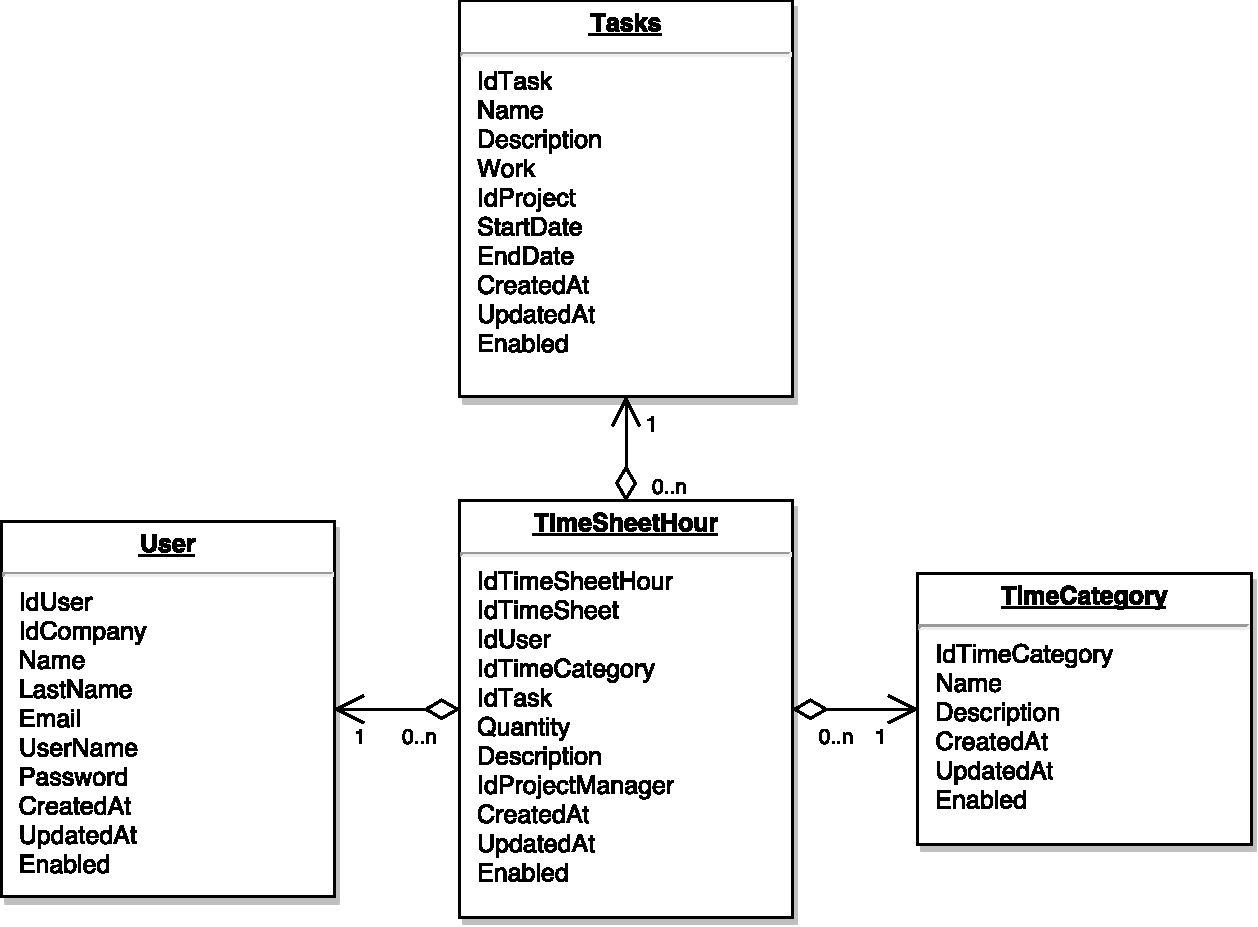
\includegraphics[width=0.8\textwidth]{Bilder/Diagramm.pdf} 
	\caption{Diagramm eines Software Designs}
	\label{fig:Diagramm-DrawIo}
\end{figure}

Ein weiteres kostenloses Tool für die Darstellung von Klassendiagrammen oder auch Sequenzdiagrammen ist \textbf{\href{http://staruml.io/}{StarUML}}. Dieses generiert auch SVG Dateien, welche du mithilfe von Inkscape zu PDF Dateien konvertieren kannst.

%\chapter{Mathematik}

\section{Text}
Hier steht ein beispielhafter Text bei dem nun auf eine sehr bekannte und durchaus vertraute Formel im Text direkt mit $c = \sqrt{a^2 + b^2}$ eingegangen wird. Dabei können auch Winkel wie: $\alpha, \beta, \gamma$ gerne verwendet werden. Weiterhin werden hier nur Formeln im Bereich der $\mathbb{N}$ dargestellt, gerne können diese aber durch Formeln aus diesem Bereich der $\mathbb{R}$ ergänzt werden.

\section{Formeln}
Beachte bei Formeln keine konkreten Werte anzugeben, sondern die Formel stets nur wie in der Literatur nur als Größengleichungen anzugeben.
\begin{align}
	\sum_{n=0}^{\infty}x=b+n\\
	\frac{b*x}{c} = y
\end{align}

Trotz unterschiedlicher Länge kann man die Gleichheitszeichen auf der gleichen Höhe anbringen wie in \autoref{eq:Gleichung1} und \autoref{eq:Gleichung2} dargestellt, zusätzlich kann man diese auch mit Informationen versehen wie in Formel \autoref{eq:Gleichung3} zu sehen.

\begin{align}
	\label{eq:Gleichung1} a + b &= c\\
	\label{eq:Gleichung2} 5c + 3f &= 4h\\ 
	\label{eq:Gleichung3} \overbrace{5y}^{y = 0} + \underbrace{42x}_{x = 1} &= b
\end{align}

\section{Arrays und Matrizen}

\begin{center}
	\(
	\begin{array}{lc|r}
		a&b&c\\
		\hline
		x&y&z\\
		c&a&b
	\end{array}
	\)
\end{center}

\begin{equation}
	\begin{array}{lcl}
		z & = & a \\
		a + b & = & c \\
		f(x,y,z) & = & x + y + z
	\end{array}
\end{equation}

Hier noch ein paar Matrizen Beispiele in \LaTeX{}.

\begin{align}
	\begin{pmatrix}
		a_{11}	& \dots   & a_{1n}\\
		\vdots	& \ddots  & \vdots\\
		a_{n1}	& \dots   & a_{nn}\\
	\end{pmatrix}
	\\[0.4cm]
	\begin{bmatrix} 
		100&250\\
		300&499
	\end{bmatrix}
	\\[0.4cm]
	\begin{Bmatrix} 
		100&250\\
		300&499
	\end{Bmatrix}
	\\[0.4cm]
	\begin{Vmatrix}
		100&250\\
		300&499
	\end{Vmatrix}
\end{align}

\section{Klammern und Kästchen}

\begin{center}
	\( \Vert x\Vert_{p}=
	\left(
	\sum_{i=1}^{n} | x_{i} |^{p}
	\right)^{\frac{1}{p}} \)
\end{center}

\begin{center}
	\( \left.
	\begin{array}{lc|r}
		a&b&c\\
		\hline
		x&y&z\\
		c&a&b
	\end{array}
	\right\}
	\Rightarrow z,b \)
\end{center}

\begin{equation*}
\mbox{
	\boxed{
		\sin^2\varphi+\cos^2\varphi=1
	}
}
\end{equation*}


%\chapter{Programm- bzw. Quellcode}
\section{Quellcode}
Ein wichtiger Punkt ist auch, dass man Quellcode Stücke mit in seinen Praxisbericht einbaut. Hier nun einfach mal ein Beispiel in Form eines kleinen JAVA Codes, welcher aus einer Datei gelesen wird:

\lstinputlisting[
	label=code:algQuersumme,    % Label; genutzt für Referenzen auf dieses Code-Beispiel
	caption=Algorithmus zur Berechnung der Quersumme,
	captionpos=b,               % Position, an der die Caption angezeigt wird t(op) oder b(ottom)
	style=EigenerJavaStyle,     % Eigener Style der vor dem Dokument festgelegt wurde
	firstline=3,                % Zeilennummer im Dokument welche als erste angezeigt wird
	lastline=18                 % Letzte Zeile welche ins LaTeX Dokument übernommen wird
]{Quellcode/Eigenes-Java-File.java}

Zu beachten ist, dass jedes Stück Code kommentiert werden sollte. Was wird in diesem Abschnitt genau durchgeführt. Wo könnten Probleme auftreten und warum wurde dieses Stück hier hinzugefügt.

\vspace*{0.5cm}

\pagebreak
\textbf{EVENT 01} \textit{INIT}
\lstinputlisting[
	label={code:SSCUI-AfterInit},  % Label; genutzt für Referenzen auf dieses Code-Beispiel
	caption={Initialisierung im Programm},
	captionpos=b,               % Position, für die Caption:  t(op) oder b(ottom)
	style=EigenerABAPStyle,     % Eigener Style der vor dem Dokument festgelegt wurde
	firstline=4,                % Zeilennummer im Dokument welche als erste angezeigt wird
	lastline=23                 % Letzte Zeile welche ins LaTeX Dokument übernommen wird
]{Quellcode/Eigenes-ABAP-File.abap}

Es ist auch möglich, innerhalb des Listings \LaTeX{} Befehle zu verwenden. Dazu muss aber eine Escape-Sequenz angegeben werden. Das folgende Beispiel enthält ein Label, auf das dann verwiesen werden wird: Auch hier funktioniert \texttt{\textbackslash{}autoref}: \enquote{In \autoref{code:var_b} wird der Variable \texttt{b} \ldots}.

\begin{lstlisting}[
  style=EigenerJavaStyle,
  captionpos=b,
  caption={Zuweisung von Variablen},
  label={code:basic_block},
  escapeinside={@}{@}]
int a = 10;
@\label{code:var_b}@int b = a + 20;
return;
\end{lstlisting}

\pagebreak
Weitere Programmiersprachen können auch eingebunden werden. Hier mal ein Beispiel in der Programmiersprache Python:
\lstinputlisting[
	label=code:WhileLoop,    % Label; genutzt für Referenzen auf dieses Code-Beispiel
	caption=Algorithmus zum Schätzen einer Zahl in Python,
	captionpos=b,               % Position, an der die Caption angezeigt wird t(op) oder b(ottom)
	style=EigenerPythonStyle,   % Eigener Style der vor dem Dokument festgelegt wurde
	firstline=0,                % Zeilennummer im Dokument welche als erste angezeigt wird
	lastline=23                 % Letzte Zeile welche ins LaTeX Dokument übernommen wird
]{Quellcode/Eigenes-Python-File.py}

\clearpage % Absichtlicher Seitenumbruch, um ein besseres Layout zu erhalten.

\section{Pseudocode}
Pseudocode kann hilfreich sein, wenn \enquote{richtig} implementierte Algorithm in einer Programmiersprache zu lang sind und diese mittels Pseudocode bündig zusammengefasst werden können. \autoref{lst:euclid} zeigt Pseudocode.

Die Doku für das Package und damit eine Liste aller Befehle findet sich unter \newline
\url{http://tug.ctan.org/macros/latex/contrib/algorithmicx/algorithmicx.pdf}

\begin{algorithm}
	\caption{Euclid's algorithm}\label{lst:euclid}
	\begin{algorithmic}[1]
		\Procedure{Euclid}{$a,b$}\Comment{The g.c.d. of a and b}
			\State $r\gets a\bmod b$
			\While{$r\not=0$}\Comment{We have the answer if r is 0}
				\State $a\gets b$
				\State $b\gets r$
				\State $r\gets a\bmod b$
			\EndWhile\label{euclidendwhile}
			\State \textbf{return} $b$\Comment{The gcd is b}
		\EndProcedure
	\end{algorithmic}
\end{algorithm}

%\chapter{Literaturhinweise}

\textbf{Hinweis}: Verwendest du eine Quelle nicht, dann nimmt \LaTeX{} diese nicht mit ins Literaturverzeichnis auf!

\section{Fußnoten und Literaturverweise}
Hamburger, Döner, Currywurst\footnote{Hier fehlt eindeutig das Lieblingsessen der Informatiker, die Pizza!} - jeder kennt sie, jeder liebt sie und jeder isst sie.
Weil die Zeit drängt\cite{Bonnen.2016}, der Hunger groß ist und der nächste Schnellimbiss\cite{Forsthuber.2016} nur drei Schritte voraus. Und nach dem Essen?
Sind wir zwar satt, aber meist nicht wirklich glücklich, weil Fastfood\cite{Friedl.2017} meist eben auch nicht wirklich gut ist \cite{Kuhnlein.2016}.

Ja, uns ist bewusst, dass die Literatur nicht zum Text passt.
Deswegen hier nochmals der Rest.\cite{Mukherjee.2017, Preuss.2017, Schell.2017, Smith.2017, Visser.2017, Zaidi.2017, o.V..o.J.}

Übrigens: \acfp{ISBN} gehören nicht in die Bibliographie und werden deshalb auch nicht angezeigt.


\chapter{Introduction}
\section{Motivation}
\subsection{Current situation}
\subsection{Importance}
\section{Research Question}
\section{Outline}
\chapter{Objectives and Criteria}
\section{Detailed Task Description}
The goal of the thesis is to add value to real business documents by aggregating expenses into clusters of similar expenses. The supplied document dataset consists of 150.000 invoices. The invoices contain different information, for example the vendor, billing amount or a description of the goods. Valuable information for companies would be insight into the different categories of expenses and the corresponding cost. With traditional data analysis methods, the company’s controlling departments cannot identify which expenses are similar in nature (for example logistics costs). 

The task is to perform a full data analysis on the supplied dataset. The dataset is to be prepared for processing with established methods. An evaluation for different means of feature extraction, machine learning, model evaluation and visualization should be performed. With the evaluation a complete flow for the data processing should be presented. The result should be an added value to the dataset in the form of aggregated expenses.

\section{Criteria set by SAP SE}
none?

\section{Research Model}
To solve the task described in chapter 1.2, this paper employs the \ac{CRISP-DM} \cite{CRISPDM2000}. This model puts forward a structure for conducting data mining projects. \ac{CRISP-DM} was developed in 1996 by three companies, which are now the partners of the \ac{CRISP-DM} consortium: NCR, DaimlerChrysler AG and SPSS Inc. 

\begin{figure}[ht]
	\centering
	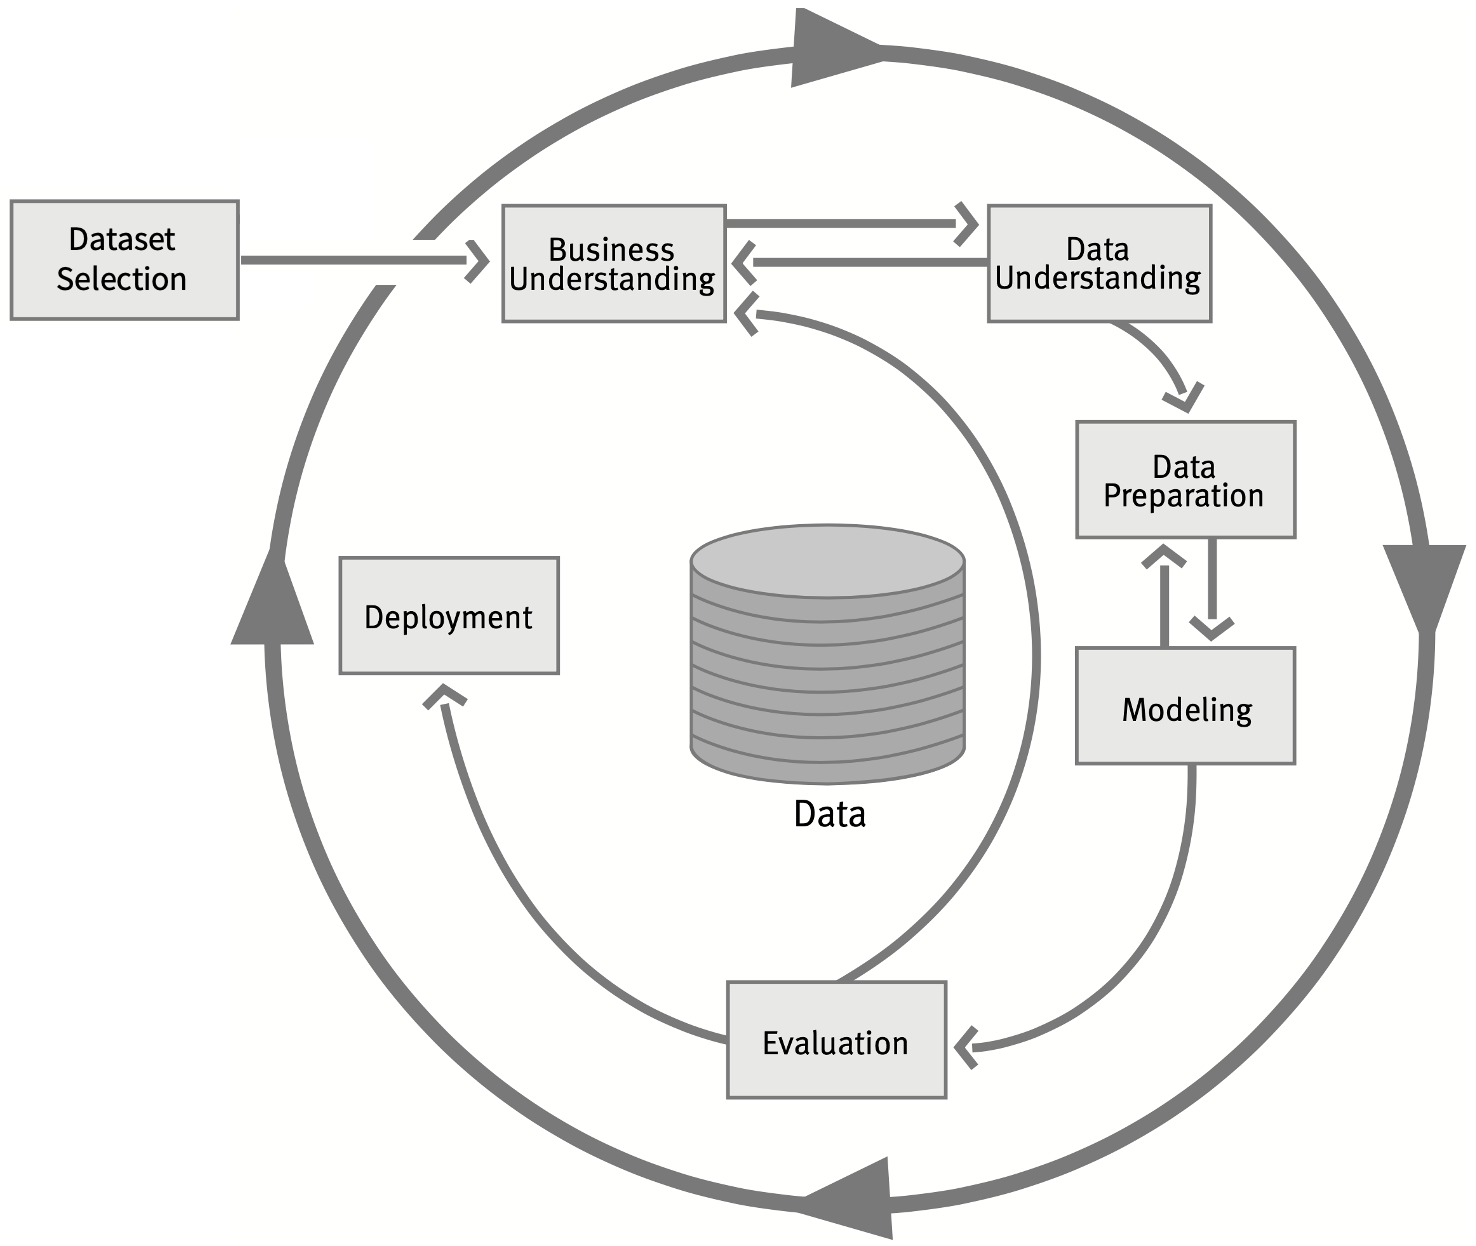
\includegraphics[height=10cm]{Bilder/Research_Model.png}
	\caption{Adjusted CRISP-DM Model}
	\label{fig:CRISM-DM}
\end{figure}

Classically, the reference model consists of six phases: Business Understanding, Data Understanding, Data Preparation, Modeling, Evaluation, and Deployment. For this thesis the model was adapted to reflect all tasks encompassed. The phase "Dataset Selection" was added, resulting in a total of seven phases.

Fundamentally, the \ac{CRISP-DM} model is of circular nature, reflecting the fact that data science projects underly the premise of continuous improvement. After the deployment of one solution, monitoring can give insights which allow for deeper business understanding, triggering the start of a new circuit of the model.




- what does the model describe?

- what are the steps?

- why do I use this model?

- Which alterations were made?
 
\chapter{Fundamentals}
\section{Glossary of Terms}

\section{Corporate Environment}
\section{Machine Learning}
Already Alan Turing understood that for laymen a learning machine can be perceived as a paradox.  How can a machine learn, if a human has to define its behavior beforehand? There are three major subfields in the discipline of artificial intelligence that fundamentally explain how a computer can learn how to behave despite predefined behavior.

\subsection{Supervised Learning}
A supervised learning algorithm learns its decision with the help of a data set (input) that also contains the correct decision (output) as information. It is trained with only a part of the entire data set, so that the model can be tested in a later step with the help of unknown data. This way, a statement can be made about the accuracy of the model.

\subsection{Unupervised Learning}
Unsupervised learning is complementary to supervised learning. All algorithms that fall into the category of unsupervised learning are trained with data that does not contain the correct output (label) as information. Here, the categorization is not constrained by the given data, but decided on by the algorithm.

\subsection{Reinforcement Learning}
The third way in which an algorithm can make better decisions as it gains experience is called reinforcement learning. Reinforcement learning is about letting algorithms solve very complex tasks. The special feature is that there is no defined solution path, but the algorithm is rewarded for goal-oriented behavior and punished for wrong decisions. The definition of goal-oriented behavior has to be put into place by the engineers setting up the training of the model. Real-world tasks are extremely complex, so not all possible solution paths can be calculated and compared to find the optimal path. Parking a car is a routine task for a human after a few hours of driving, but a computer sees only an infinite set of possibilities for turning angles. This problem can be solved by reinforcement learning. The algorithm is rewarded for each parking attempt where the car ends up seeing in the parking space. For the remaining attempts, the algorithm is penalized. Over many thousands of attempts, the reinforcement learning model is trained in this way.

The three major ways of learning even with previously defined behavior can now be implemented by specific models. For example, there are several ways to create and train a model using Unsupervised Learning.

\section{Natural Language Processing}
\ac{NLP} is often attributed to the computer science, but after closer examination, \ac{NLP} is a discipline comprised of linguistics, computer science, artificial intelligence an mathematics \cite{gobinda_g_chowdhury_natural_2003}.

\section{SAP AI Core}
\section{Docker}


\chapter{Dataset selection}
Which datasets are available?

\section{Alternatives}

	The dataset is the fundament of a data-science project. The quality, size and closeness to reality decide the degree to which the findings can be helpful for solving real problems. 
	In this section, a classification for data-science projects is introduced.
	
	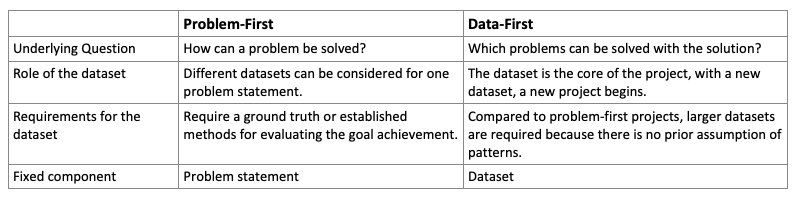
\includegraphics[height=4cm]{Bilder/meta_project.png}
	
	The problem-first project type is characterized by a predefined problem statement or research goal. The underlying question is, how a specific or a set of problems can be solved. For the selection of the dataset, this requires that goal achievement can be measured with existing ground truth. In some cases, also other methods such as expert judgements can be sufficient. In a problem-first project, different datasets can and should be considered.
	
	The complementary project type is the data-first project, which describes most data-mining projects. This type is characterized by a more explorative approach, and the goal to find problems and patterns. Here, the dataset is at the core of the project and the fixed aspect of a project. In turn, this means swapping the dataset is the start of a new project.
	
	With the project type as a decisive factor for the dataset explained, the other evaluation criteria for the dataset is described. In the corporate environment two fundamental sources for data exist. 
	
	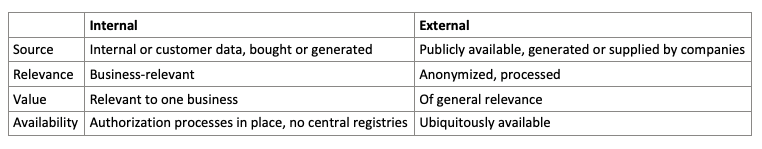
\includegraphics[height=3cm]{Bilder/internal_external.png}
	
	Firstly, data can be sourced from inside the company. This can include customer data or data generated from observation and monitoring processes inside the company. Data is either directly or very closely related to the company's business. Depending on the solution, it can be of use to customers or it can be utilized inside the company. Internally sourced data is almost exclusively rated confidential, limiting even intra-company access to it. Authorization processes and more than often not existing registries for data may hinder project progress.
	
	Secondly, data can be sourced outside the company. A vast number of online registries for data exist, both with paid and free of charge service offerings. Data sources include real-life data and data generated for educational purposes. Because of its publication, the data is stripped from all parts which could expose confidential information such as corporate secrets. Additionally, data is anonymized and processed to limit the usefulness to potential competitors.
	
	It can be stated, that both sources are suited for different goals. 

\section{Practical Implementation}
	T
\chapter{Business Understanding}
In \cite{CRISPDM2000}, different tasks, and outputs for developting a business understanding are mentioned. The task and respective output will be dicussed in the following sections.

\section{Determine Business Objectives}
Businesses without existing an \ac{ERP} solution in place can easily be overwhelmed by the number of invoices reaching them daily. Even more, the controlling department can easily lose the overview of spending. To quickly gain a perspective on the most important spending topics, spending should be sorted in categories of similar nature.

The primary goal is the development of a solution for automatic aggregation of documents, based on topics adressed in those documents. The focus is on shorter text segments, such as product descriptions. The business objective is an information gain, on how spending is distributed among cross-cutting topics in a company.

The created solution can be evaluated with the business success criterion: "Does the solution identify and give useful insights in the money pits?". This judgement of having achieved the goal is a subjective matter. Evaluating the success should therefore be distributed among several stakeholders, including but not limited to the author, the supervisor and the supplier of the data.


\section{Assess Situation}

\subsection{Inventory of Resources}
An \ref{tabelle:inventory} was created for assessing the situation. Most notably is the availability of experts through excellent intercorporational cooperation. Also, a large collection of datasets is available. Hardware platforms include personal machines as well as hosted environments with GPU capabilities. Available software are data science tools included in the Anaconda Navigator, such as Jupyter Notebook. All open-source libraries are of course also included.

\section{Determine Data Mining Goals}


\section{Produce Project Plan}
\chapter{Data Understanding}

\section{Initial Data Collection Report}

\subsection{Data Requirements Planning}
The business objective is the development of a solution for the automatic aggregation of documents based on their topics. To achieve this goal, a sufficient number of documents are required. Also, the documents must contain enough text to be assigned a topic. After clustering the value of each expense in a cluster have to be summed, to gain the desired insight of spendings in one category. So the value an expense amounts to has to be included in the data.

\subsection{Selection Criteria}
An initial look a the data has shown that each invoice item can easily contain more than 100 pieces of information, which can be considered as attributed in the dataset. The part of the data that is of interest for the research is the description and payment data. Other data needs to be retained for a coherent and informative presentation of the results, such as location information and information on seller and buyer.

\subsection{Insertion of Data}

The insertion of data is concerned with the theoretical utilization of the data and problems arising during this process. The encoding and grouping of free text items is referenced as one concern in the \ac{CRISP-DM} user guide \cite{CRISPDM2000}. In this research the focus is on free text items, therefore this step will be discussed in detail in the following chapter. 
Other concerns are missing attributes. The dataset has already undergone a surface-level evaluation, which concludes that all relevant attributes are contained.

\section{Data Description Report}
The data is available as a local folder of size 5.12 GB, it contains 152,592 \ac{JSON} files. Each \ac{JSON} represents one invoice document. 
How many features per invoice?
What are the features?
Are there correlations between the attributes?
basic statistics for each significant attribtue

\begin{figure}[ht]
	\centering
	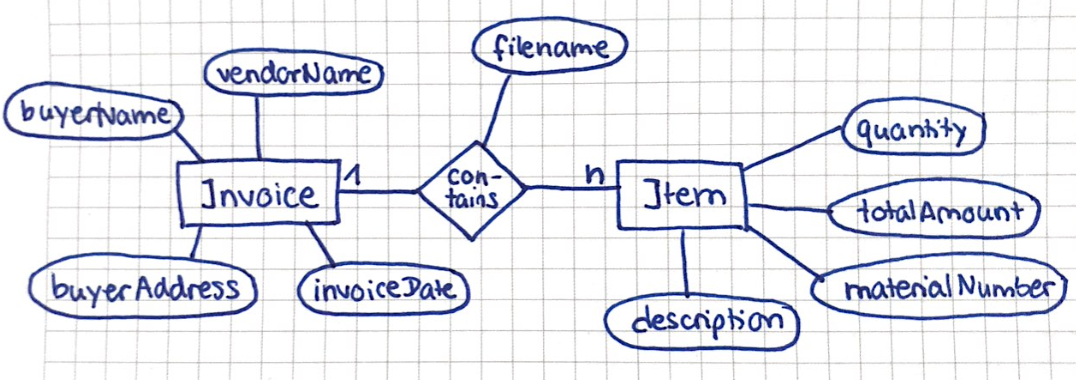
\includegraphics[height=5cm]{Bilder/practical/entity_relationship.png}
	\caption{Entity Relationship Diagram for Invoice Documents}
	\label{fig:er}
\end{figure}

\section{Data Exploration Report}
In which language are they written?
Form a hypothesis?

\section{Data Quality Report}
DOes the data contain errors?
Are there missing values?
are all values plausible?
plot some stuff here
check number of fields in each record (?) maybe optional

\chapter{Data Preparation}

	\section{Data processing and data wrangling}
	
    Data preparation is the process of transforming the acquired dataset into a dataset which can be fed into learning algorithms and is cleaned of impurities in such a way, that the learning results are likely satisfactory. Impurities may be missing values, shifted columns, encoding errors or different data formats. 
    Data preparation includes data wrangling, data cleaning, and feature extraction. What is left should be a uniform dataset, which is in a format that is understandable by the desired algorithms.
    
        \subsection{Alternatives}
        The chosen dataset consists of files in \ac{JSON}. Several alternatives for storage and transforming the data exist. 
        
        \paragraph{Storage Location}
        Within the constraints of the thesis, three options are available for data storage. Firstly, data can be stored locally on the available machine. The data is available without internet access, and the local machine has high read/write speeds. This option requires no additional learning, and is free of charge for the department. A multitude of libraries exist for accessing files on a local filesystem. A downside is the limited scalability in terms of storage capacity and read/write operations. Additionally, local storage makes the data only available to this specific machine.
        
        Storing data on a cloud filesharing system is easy to operate and free of usage-bound charges. The storage space is virtually unlimited. Accessing files on sharing platforms is feasible but tedious. The access can be shared within the company context, but everyone is subject to the limited accessibility. Using a files storage service could be of use for transferring data without a physical connection. Still, this is the only recommended use case in this context.
        
        The third option is storing the data using a specialized storage service, such as AWS S3. While the learning overhead is higher in the beginning, the scalability is a convincing argument. Billing is according to usage, but adequate because of the high connectivity with other cloud-based ML service offerings inside and outside of SAP.
        
        \begin{table}[ht]
            \centering
            \caption{Comparison of available Storage Options}
            \begin{tabular}{c|lll}
                \toprule
                &\textbf{Local} & \textbf{Cloud Filesharing} & \textbf{Specialized Storage Services} \\
                \midrule
                \vspace{0.5cm}
                Example     & \begin{tabular}[c]{@{}l@{}}2.6GHz \\ 512GB SSD\end{tabular} & Microsoft OneDrive                                                        & AWS S3                                                                                                 \\
                \vspace{0.5cm}
                Ease of use & high                                                        & high                                                                      & higher learning overhead                                                                               \\
                \vspace{0.5cm}
                Cost        & free of charge                                              & free of charge                                                            & \begin{tabular}[c]{@{}l@{}}billing according to \\ used storage space\end{tabular}                     \\
                \vspace{0.5cm}
                Scalability & limited                                                     & unlimited                                                                 & unlimited                                                                                              \\
                \vspace{0.5cm}
                Data access & local                                                       & \begin{tabular}[c]{@{}l@{}}limited remote \\ access capacity\end{tabular} & \begin{tabular}[c]{@{}l@{}}local, remote, high \\ connectivity to \\ ML service offerings\end{tabular}
                
            \end{tabular}
            \label{tabelle:storage}
        \end{table}
        
        \paragraph{Data Format}
        The data is still available only in the from \ac{JSON} documents.
        
        - transforming json documents into dataframe rows
        
    \subsection{Theoretical Implementation}
    For the data wrangling the invoices have to be read into memory and then processed into a reusable structure. Each document will be read into memory, then the necessary information will be extracted. All invoices will be combined into one data structure, which then is persisted for later use.

    \begin{figure}[ht]
        \centering
        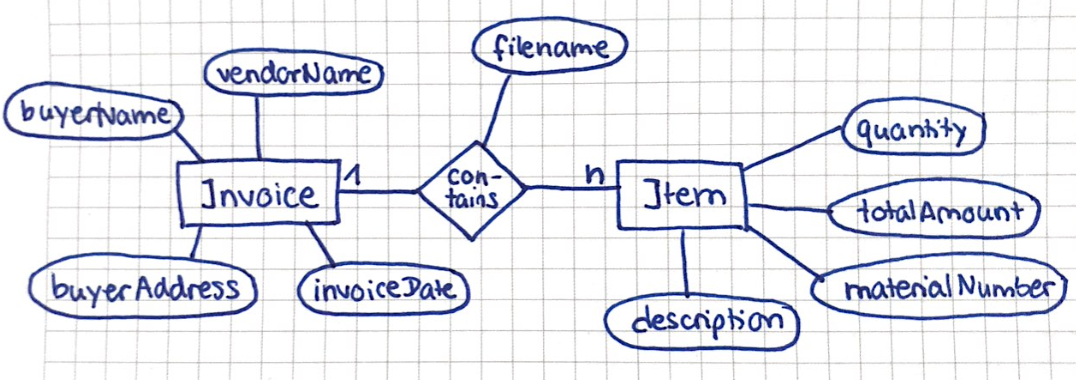
\includegraphics[height=5cm]{Bilder/practical/entity_relationship.png}
        \caption{Entity Relationship Diagram for Invoce Documents}
        \label{fig:er}
    \end{figure}

	The data for an invoice and its contained items is stored in an array of objects. This is also shown in code example (\ref{code:JSONSchema}) of a shortened JSON Schema for one invoice. The array "annotations" contains objects. One object represents information such as the invoice date or the unit price. 
	Information about invoice items have labels containing the prefix "lineItem". One invoice containing several items is represented by duplicate values of one label (in the example \ref{code:JSONInvoice} the label "lineItem.description.value"). Here, the order of the labels has to be retained during data wrangling to ensure not mixing up information about different invoice items.

	\lstinputlisting[
	label=code:JSONInvoice,    % Label; genutzt für Referenzen auf dieses Code-Beispiel
	caption=JSON of one invoice,
	captionpos=b,               % Position, an der die Caption angezeigt wird t(op) oder b(ottom)
	style=EigenerPythonStyle,   % Eigener Style der vor dem Dokument festgelegt wurde
	firstline=0,                % Zeilennummer im Dokument welche als erste angezeigt wird
	lastline=23                 % Letzte Zeile welche ins LaTeX Dokument übernommen wird
	]{Quellcode/invoice.json}
	
    \subsection{Practical Implementation}

	The files are processed in python, using the library "json". Each file is opened, and decoded with python's build in json decoder. The hierarchy is traversed until the array "annotations" is reached. Now, the tuples of label and text are saved. This process is split up into invoice and item labels.
	
	The information on invoices is stored in a tabular data structure, a python pandas DataFrame. Worth mentioning is that some invoices contain more information than others. In this case, invoices are still appended into one table, but fields for non-existent values are left empty. The filename is the unique identificator for one invoice.
	
	\begin{figure}[ht]
		\centering
		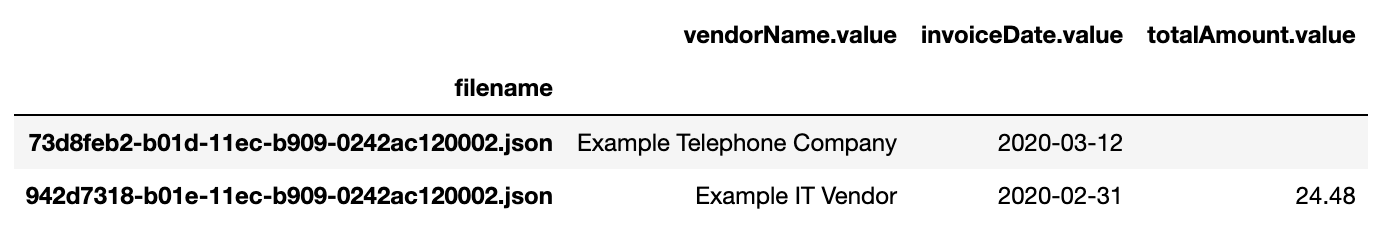
\includegraphics[height=2.5cm]{Bilder/practical/df_invoices.png}
		\caption{Exemplary depiction for processed invoices in a DataFrame}
		\label{fig:df-invoices}
	\end{figure}

	Similarly, information on the invoice items is retrieved from the documents and stored in a pandas DataFrame. Every invoice item has an unique id and can be linked to the respective invoice through the filename.
	
	\begin{figure}[ht]
		\centering
		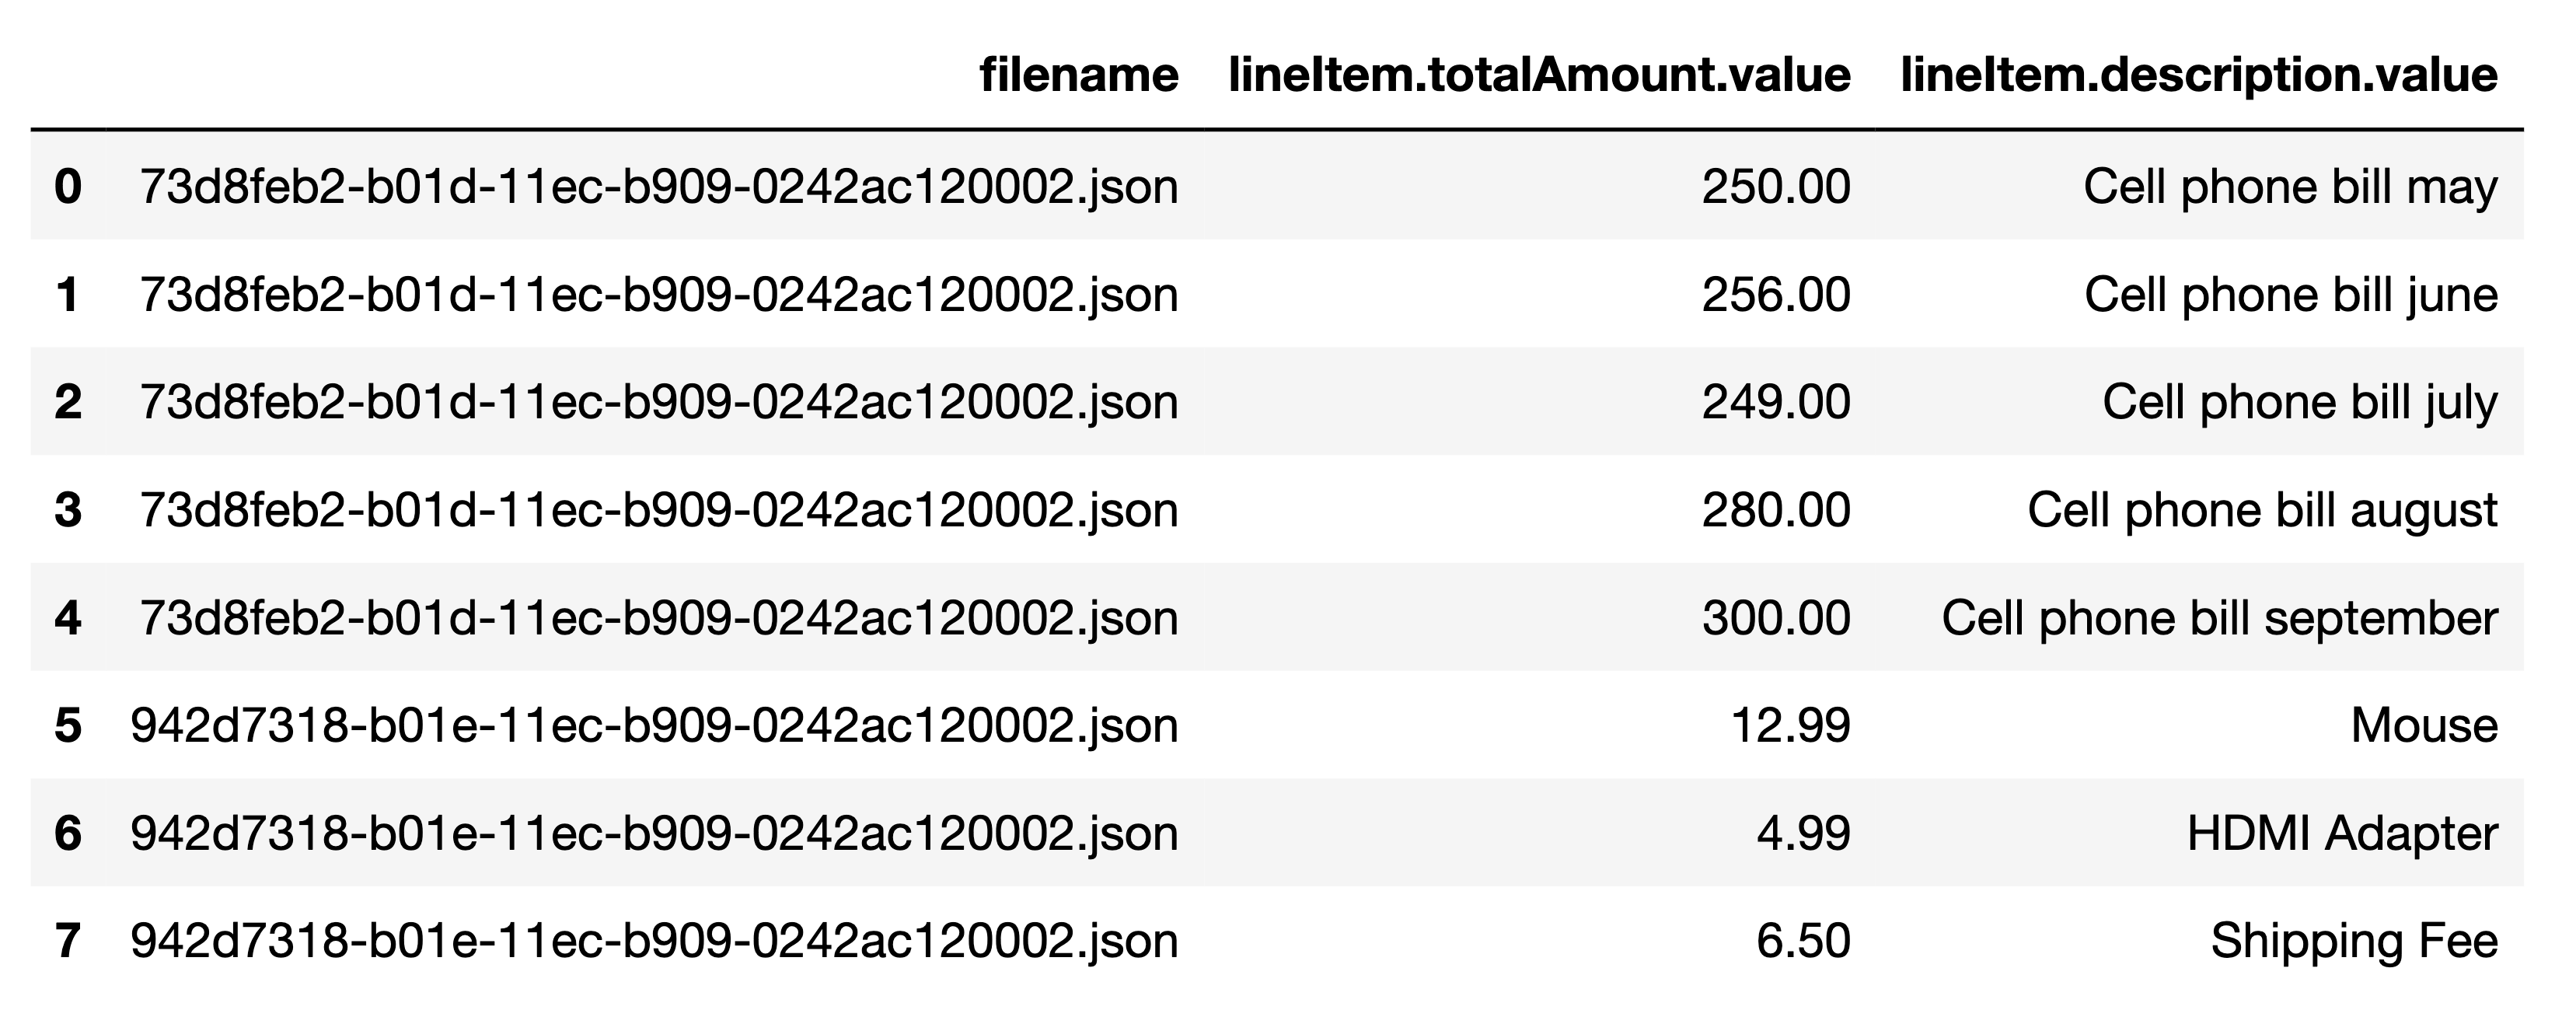
\includegraphics[height=6cm]{Bilder/practical/df_lineitems.png}
		\caption{Exemplary depiction for processed invoice items in a DataFrame}
		\label{fig:df-invoices}
	\end{figure}
	
	The resulting two DataFrames are serialized with the python standard library "pickle".  The data can be efficiently loaded into memory and reserialized again with this library.
	
	This processing step allowed for storing the initial 5.12GB of data in a more usable format and takes up only a total of 393MB. Even further improvements to storage will be dicussed later on.

	The process of reading files from the disk is not inherently an expensive one, but in the realms of many thousand documents, processing times soon reach several days. Observing the execution of the python code showed a peculiarity: While the utilization of the used processor was consequently at the maximum, only one process is executed, leaving the total CPU usage at only 20\%. 
	
	\begin{figure}[ht]
		\centering
		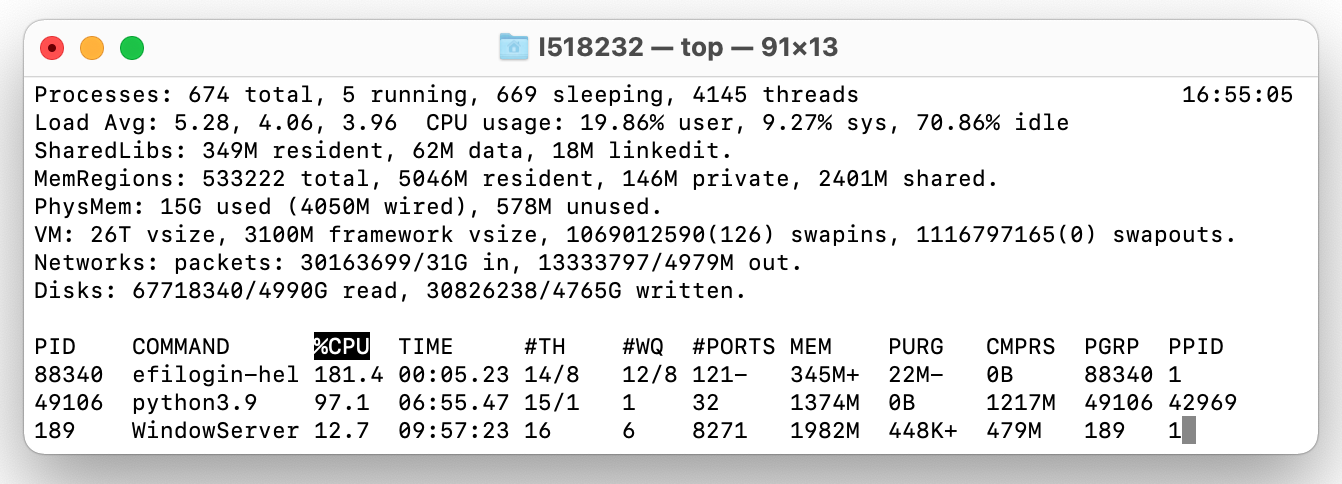
\includegraphics[height=4cm]{Bilder/practical/python_processes.png}
		\caption{Exemplary depiction for processed invoice items in a DataFrame}
		\label{fig:df-invoices}
	\end{figure}
	
	
	One question that may now arise is: Why doesn't python split up the workload and employ the full capacity of the machine?
	This can be explained with the design of the Python interpreter. The \ac{GIL} controls access to the Python Virtual Machine executing the code. This lock only allows exactly one thread to run at a time \cite{corePython}. This of course is not favorable, as valuable CPU capacity is unused. Fortunately, the \ac{GIL} behaves in a special way regarding C code, and I/O operations in Python utilize C code: the lock is released before executing a C routine \cite{corePython}. This allows to bypass the (in this case) inconvenient locking mechanism. 
	
	Different python libraries exploit this speciality and allow to spawn a pool of different processes, which then execute calls asynchronously. One example is the ProcessPoolExecutor. A notable restriction is that only picklable objects can be submitted for multiprocessing. This concerns both fuction and its parameters. While this is not a problem in this task, this restriction will become important later on in the section about feature extraction.
	
	\lstinputlisting[
	label=code:JSONSchema,    % Label; genutzt für Referenzen auf dieses Code-Beispiel
	caption=Shortened JSON Schema of one invoice document representation,
	captionpos=b,               % Position, an der die Caption angezeigt wird t(op) oder b(ottom)
	style=EigenerPythonStyle,   % Eigener Style der vor dem Dokument festgelegt wurde
	firstline=0,                % Zeilennummer im Dokument welche als erste angezeigt wird
	lastline=23                 % Letzte Zeile welche ins LaTeX Dokument übernommen wird
	]{Quellcode/json-schema.json}
	
	

	
	\section{Data cleaning}
    - removing stopwords from several languages
        
    - removing numbers and interpunction
    
    - tokenization
	The task of data cleaning was also completed using python scripts. The library \ac{NLTK}
	
	\begin{lstlisting}[language=sh]
$ python3 -c 'import cleaner; print(cleaner.clean("500grams of special baking flour type 504"))' 
>>>  ['of', 'special', 'baking', 'flour', 'type']
	\end{lstlisting}
	 
	\section{Considerations of Space and Time Complexity}
	The dataset consists of over 150.000 invoices, and in those invoices, over 350.000 items are listed. 
	With hardware-limitation in place, an optimized approach for storing and processing the data is required. 
	Several considerations for speeding up processing time and reducing storage space can be made. 
	In the following, the observations are explained and approaches for improvement are given.

		\subsubsection{Duplicates and space complexity}
		Investigation shows, there are only 79.741 unique descriptions for the listed items. By saving only the unique values, the required space is reduced to less than one fourth compared to before. Additionally, this step is required by most machine learning models, as duplicate input values can skew the outcome. The model is chosen later, so this processing step leaves the model selection more open to different kinds of learning algorithms.
		
		\subsubsection{Reconstructing Relationships and time complexity of searching}
		After the deletion of duplicate descriptions (documents in the corpus), the 
		
		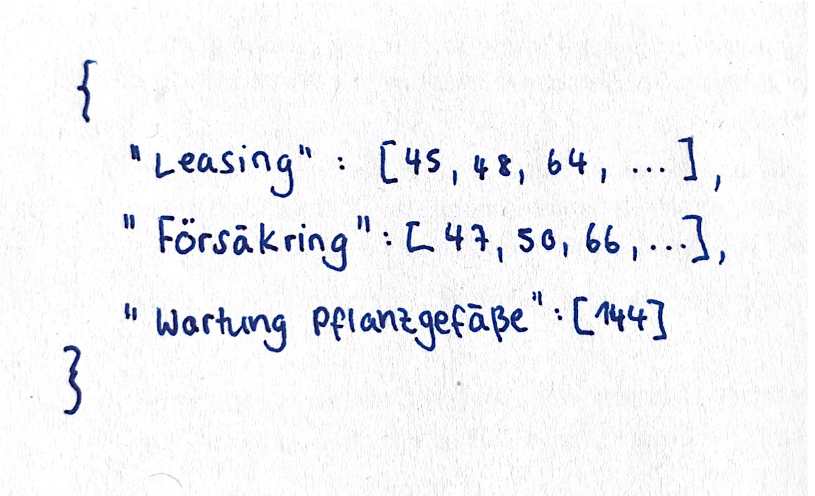
\includegraphics[height=8cm]{Bilder/description_map.png}

Explain how I want to store the data. Explain the successive artifacts.

        
        \section{Feature Extraction and Feature Engineering}
        The majority of pupular ML algorithms require the input of scalar, vector or matrix data. A form of ML models, which work with textual input will be discussed later in this section. 
        But since many algorithms were not designed to work with textual data, a transformation is required before already existing algorithms can be applied. Several methods for representing text as mathematical object will be discussed in the following.
    
            \subsection{Alternatives}
            \subsubsection{One-hot encoding}
            
    
            \subsubsection{Bag of Words Model}
            Following three documents will be considered to explain the workings of the \ac{BoW} model:
    
            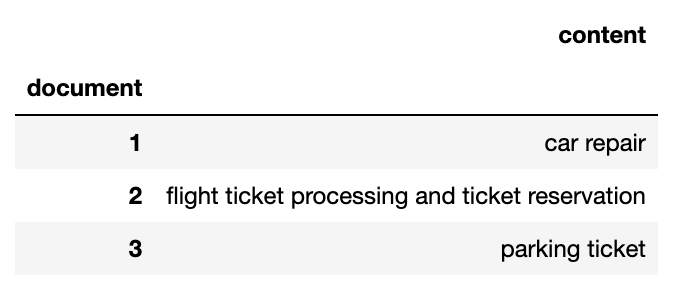
\includegraphics[height=3cm]{Bilder/corpus_bow.png}
            
            A corpus is transformed into the \ac{BoW} representation in two steps. 
            
            Firstly, the vocabulary is determined. 
            The vocabulary is a collection of all words occuring in the corpus. Every word is contained exactly once, regardless of the actual number of occurrences. The vector represenation of one document is of the same length as the vocabulary. One document being represented by one vector, a corpus of several documents can be represented as a matrix. The resulting matrix has the size $ |D|*|V| $, with $|D|$ being the number of documents in the corpus, and $|V|$ being the size of the vocabulary.
            
            Secondly, for each combination of one document $ d_{i} $ and one word $ v_{j} $ in the vocabulary, the occurrences are counted. The times, how often the specific word is contained in the document is noted in the matrix at location$  ij $.
            
            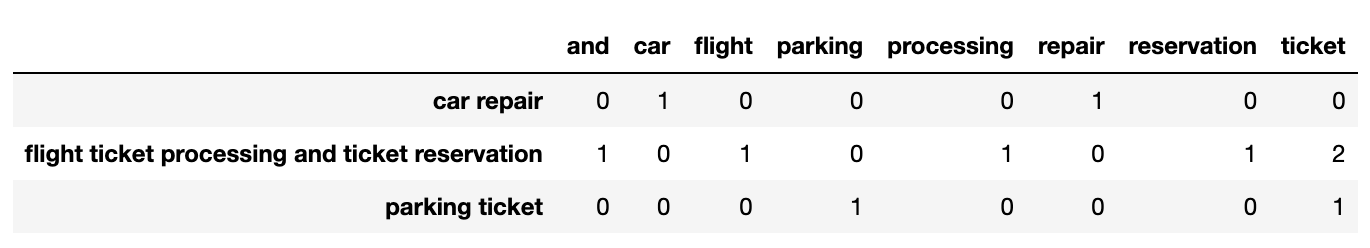
\includegraphics[height=2.9cm]{Bilder/bow.png}
    
            The result of vectorization are three vectors:
            \[ d_{1} = [0,1,0,0,0,1,0,0] \]
            \[ d_{2} = [1,0,1,0,1,0,1,2] \]	
            \[ d_{3} = [0,0,0,1,0,0,0,1]\]
    
    
            This vectorization method can be implemented with ease and in a computationally efficient manner. The \ac{BoW} model allows for a very intuitive understanding of documents, since texts consisting of the same words are considered topically related. 
            
            One of the drawbacks of this method is that no consideration is paid to words being repeated in one document. Additionally, no semantic relationship between words or documents can be inferred. 
            Further, it can be stated, that the \ac{BoW} representation fails to capture the meaning of synonyms. This becomes obvious with an example: document $ d_{1} $ and $ d_{3}$ would be considered to belong into the topic of transportation or automotives. The \ac{BoW} representation suggests topical proximity between document $ d_{2} $ and $ d_{3}$ , through the shared word "ticket". "Ticket" here is used in both the meaning of an entrace pass ($d_{2}$) and in the meaning of a note for a traffic offence  ($d_{3}$). 
            
            To conclude, the \ac{BoW} model is a straightforward text representation method. Still, it fails to capture several aspects of the natural language.
            
            \subsubsection{Tf-Idf}
            The \ac{TF-IDF} model aims to capture more meaning from the corpus by considering the composition of the whole corpus for the calculation of individual document vectors.
            
            \ac{TF-IDF} makes two assumptions about natural language:
            
            \subparagraph{1 Term Frequency}
            
            A word $t_{i} $ which occurs very frequently in one document is considered to describe a text very well. The occurences of one word in one document is denoted as $ \#( t_{i}) $.
            One additional consideration needs to be made regarding the document length. In a document of length $ |d_{2}| = 6 $ and a document of length  $ |d_{3}| = 2 $, the word $ t_{i} $occuring once would be considered equally important to each document. Of course, the word should be considered more important to $ d_{3} $, since it accounts for a larger share of the text. The measure resulting from both ideas is the term frequency:
            
            \[ TF(t_{i}, d_{j}) =   \dfrac{\#( t_{i})}{|d_{j}|} = \dfrac{occurences \; of \; word \; t_{i} \: in \; document \;\:   d_{j}}{legth \; of \; d_{j}} \]
            
            \subparagraph{2 Inverse Document Frequency}
            A word $t_{i} $ which occurs in a large number of documents does not describe one document well. Words occuring in many documents often are articles or pronouns (stopwords) which do not provide value when inspecting the content of a text. The inverse document frequence is a measure accounting for this fact. The inverse document frequency of a word is the proportion between the number of documents in the corpus and the number of documents containing the word. The logarithm is applied, as the importance of a word does not increase proportionally to the number of occurrences.
        
            
            \[ TF(t_{i}, d_{j}) = \log \dfrac{|D|}{\#(d_{t_{i}}) } =  \log \dfrac{number \;  of\;  documents \;  in \; corpus \; D}{ number \; of \; documents \; containing \; word \; t_{i}} \]
            
            Combining both assumptions, the \ac{TF-IDF} measure is created:
            
            \[ TFIDF(t_{i}, d_{j}) \;=\; TF(t_{i}, d_{j}) * TF(t_{i}, d_{j})\]
            
            For the corpus displayed in the previous section the document vectors calculated with the \ac{TF-IDF} measure are:
            
                    
            \begin{align}
                &d_1 = & [ 0\;	&0.707107\;	0\;	0\;	0\;	0.707107\;	0\;	0 \\
                &d_2 = & [ 0.39798\;	&0\;	0.39798\;	0\;	0.39798	0\;	0.39798	0.605349 
            \end{align}
                
                \[d_1 = \begin{bmatrix} 0\;	0.707107\;	0\;	0\;	0\;	0.707107\;	0\;	0 \end{bmatrix}	 \\
                d_2 =  \;\begin{bmatrix} 0.39798\;	0\;	0.39798\;	0\;	0.39798	0\;	0.39798	0.605349 \end{bmatrix} \\
                d_3 = \;\begin{bmatrix} 0\;	0\;	0\;	0.795961	0\;	0\;	0\;	0.605349 \end{bmatrix} \]
                
            The \ac{TF-IDF} measure corrects some of the pitfalls of the \ac{BoW} model. It certainly is less vulnerable to skewing by stopwords as words are ranked by importance to each document and the all over corpus. 
            
            Just as the \ac{BoW} representation, \ac{TF-IDF} suffers from high-dimensionality. The vectors contain one element for each word in the vocabulary, resulting in vectors which are inefficient to handle.
            Also, \ac{TF-IDF} fails to represent the topical relationship between $ d_{1} $ and $ d_{3}$. 
            
            \subsubsection{Word Embeddings}
             Again, the most desirable vector representation consists of dense low-dimensional vectors which are close to each other if the words are considered similar. The lack of "understanding" of related words, and the problem of high-dimensionality is corrected with the third presented option: Word Embeddings.
            
            An embedding is a translation of a word into a high-quality vector. The model does so, as it has been trained on a large set of natural language data. Popular embeddings include word2vec, fasttext and doc2vec. Word2Vec is the original model and will be discussed in the following. 
            
            The word2vec model assumes that words appearing in a similar context are also similar to each other. There are two options for the input and output: the word $w_i$ and its context $c_i$.
            
            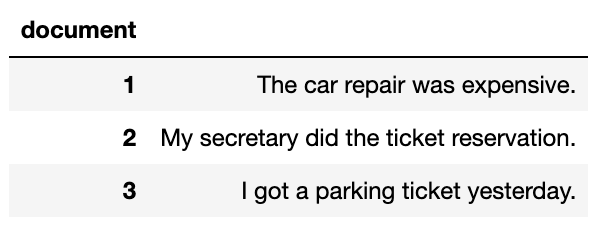
\includegraphics[height=4cm]{Bilder/word2vec/documents.png}
            
            \subparagraph{\aclu{CBOW}} 
            With the \ac{CBOW} architecture the word2vec model is trained to predict a word using the context as input. A sliding window of a predefined size is moved along the text. 
            
            \begin{figure}[ht]
                \centering
                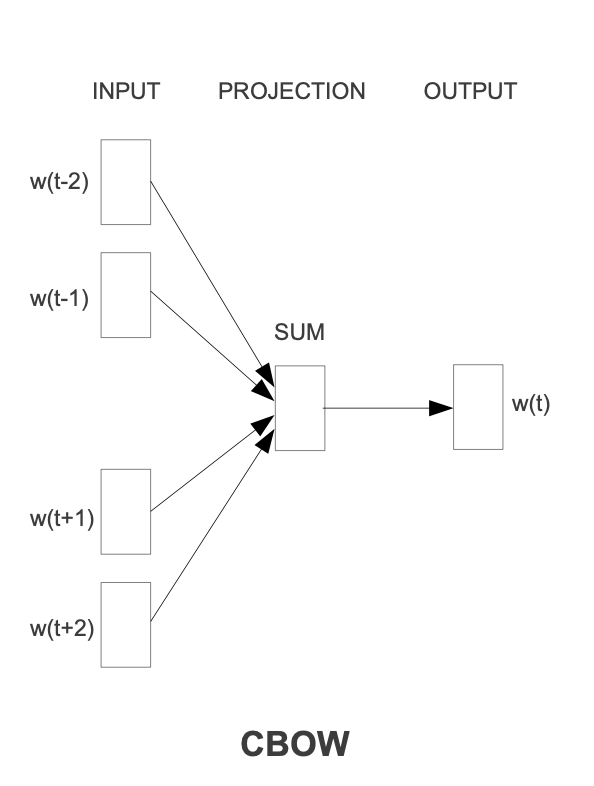
\includegraphics[height=6cm]{Bilder/word2vec/architecture_cbow.png}
                \caption{\aclu{CBOW} architecture\\\ with sliding window of size $C=5$ }
                \label{fig:cbow-architecture}
            \end{figure}
        
            \subparagraph{Skipgram} 
            With the skipgram architecture the word2vec model is trained to predict the context of the input word.
            
            \begin{figure}[ht]
                \centering
                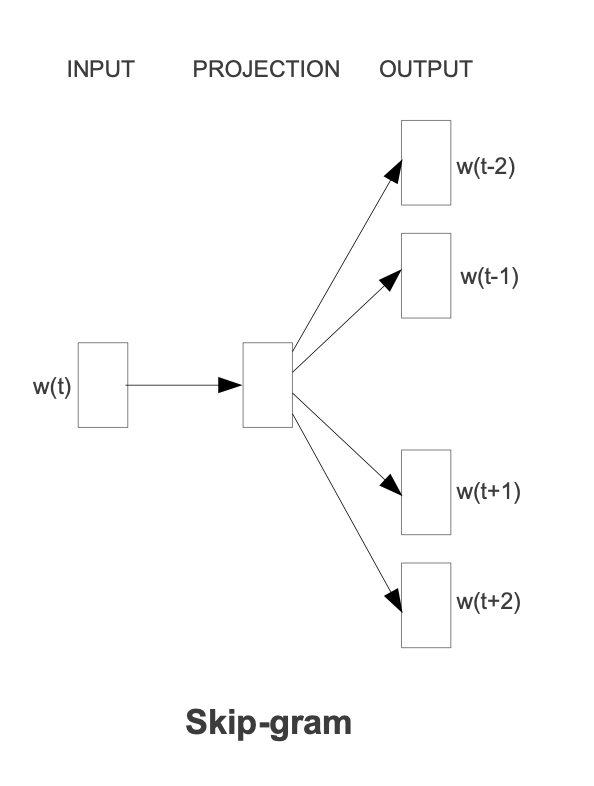
\includegraphics[height=6cm]{Bilder/word2vec/architecture_skipgram.png}
                \caption{Skipgram architecture\\\ with sliding window of size $C=5$ }
                \label{fig:cbow-architecture}
            \end{figure}
        
            \begin{figure}[ht]
                \centering
                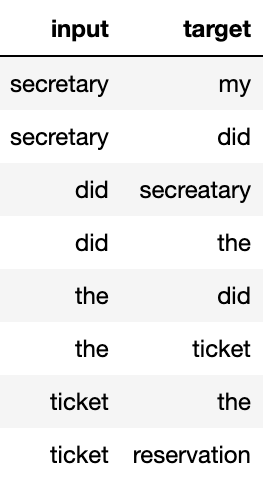
\includegraphics[height=8cm]{Bilder/word2vec/skipgram.png}
                \caption{Observations for training with skipgram architecture}
                \label{fig:cbow-architecture}
            \end{figure}
            
            
            \subparagraph{Negative Sampling}
            
            
            Word2Vec uses either SKIPGram or CBOW.
            
            Word2vec can utilize two models for selecting observations: either skipgram or \ac{CBOW}. 
            
            \subsection{Theoretical Implementation}
            
            \subsection{Practical Implementation}
            Tf-Idf weighed USEM Word vectors
\chapter{Modeling}
The objective of this thesis is the grouping of expenses with the methods of \ac{NLP}. Grouping, or clustering, is the practise of sorting data points into groups in such a way that the similarity inside a group (intra-cluster similarity) is high while the similarity between clusters (inter-cluster similarity) is low. The defintion of similarity as well as different clustering algorithms are presented and contrasted in the following sections.


\section{Alternatives}
\subsection{Similarity and distance measures}
A distance measure is a quantification of how near objects in space are. Distance measures can be defined for spaces of arbitrary numbers of dimensions. In the examples, four words (man, woman, king, queen) are compared in their semantic similarity. The word vectors were generated with a word embedding, but the focus is on comparing the distance measures available for clustering later on.

		\begin{figure}[!h]
			\centering
			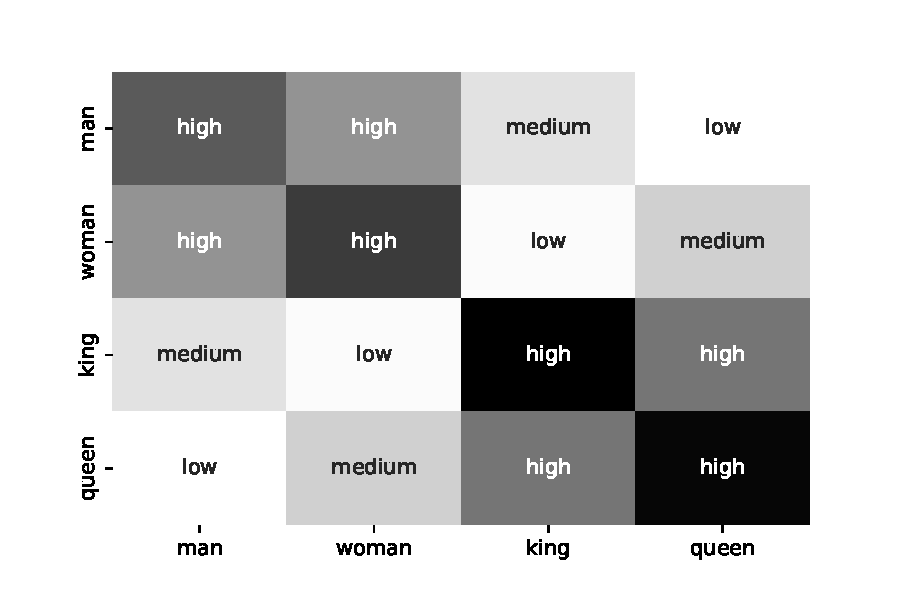
\includegraphics[height=6cm]{Bilder/models/heatmap_dot_product.pdf}
			\caption{Dot Product as Similarity Measure}
			\label{fig:dotproduct-heatmap}
		\end{figure}
	
		\subparagraph{Dot Product}
		The dot product is an operation transforming a vector into a scalar through multiplying the vectors element-wise. This operation is easily and efficiently calculated, but has some pitfalls.
		While every word in the example (\ref{fig:dotproduct-heatmap}) ranks very high in similarity to itself, the distance between the word and itself is not always the same for every word. This happens because the dot product is not agnostic of a vector's magnitude. A vector's product with itself is the square of its magnitude. This results in the similarity of man-man to be lower than the similarity of queen-queen.
		This fact makes the dot product impractical for accurately representing the relationships of words.
	
					\[ 
				\text{dot product} :=  \mathbf{A} \cdot \mathbf{B}= \sum\limits_{i=1}^{n}{A_i  B_i} 
				\]

	
		\subparagraph{Euclidean Distance} \label{euclidean}
		For low-dimensional applications, this distance works well and shows great results. Euclidean distance can be calculated in a highly efficient manner, even for n dimensions. This suggests, that euclidean distance is particularly suitable for high-dimensional data. Unfortunately, euclidean distance falls victim to the curse of dimensionality. In \cite[p.~1]{beyerNearestNeighbor} it is proven that with increasing dimensions, the distance between data points approaches an uniform value for all data points. This effect could be demonstrated for spaces with as little as ten dimensions. Therefore, it can be said that euclidean distance is not suitable for high-dimensional data. With vectors in \ac{NLP} ranging from 100 to 800 dimensions with embeddings and hundreds of thousands with \ac{TF-IDF}, this distance measure is not suitable.
		
				\[ 
		\text{euclidean distance} :=  \sum\limits_{i=1}^{n}{(A_i -  B_i)^{2}} 
		\]
		
		\begin{figure} 
			\begin{minipage}{0.49\textwidth}
				\label{fig:euclidean}
				
				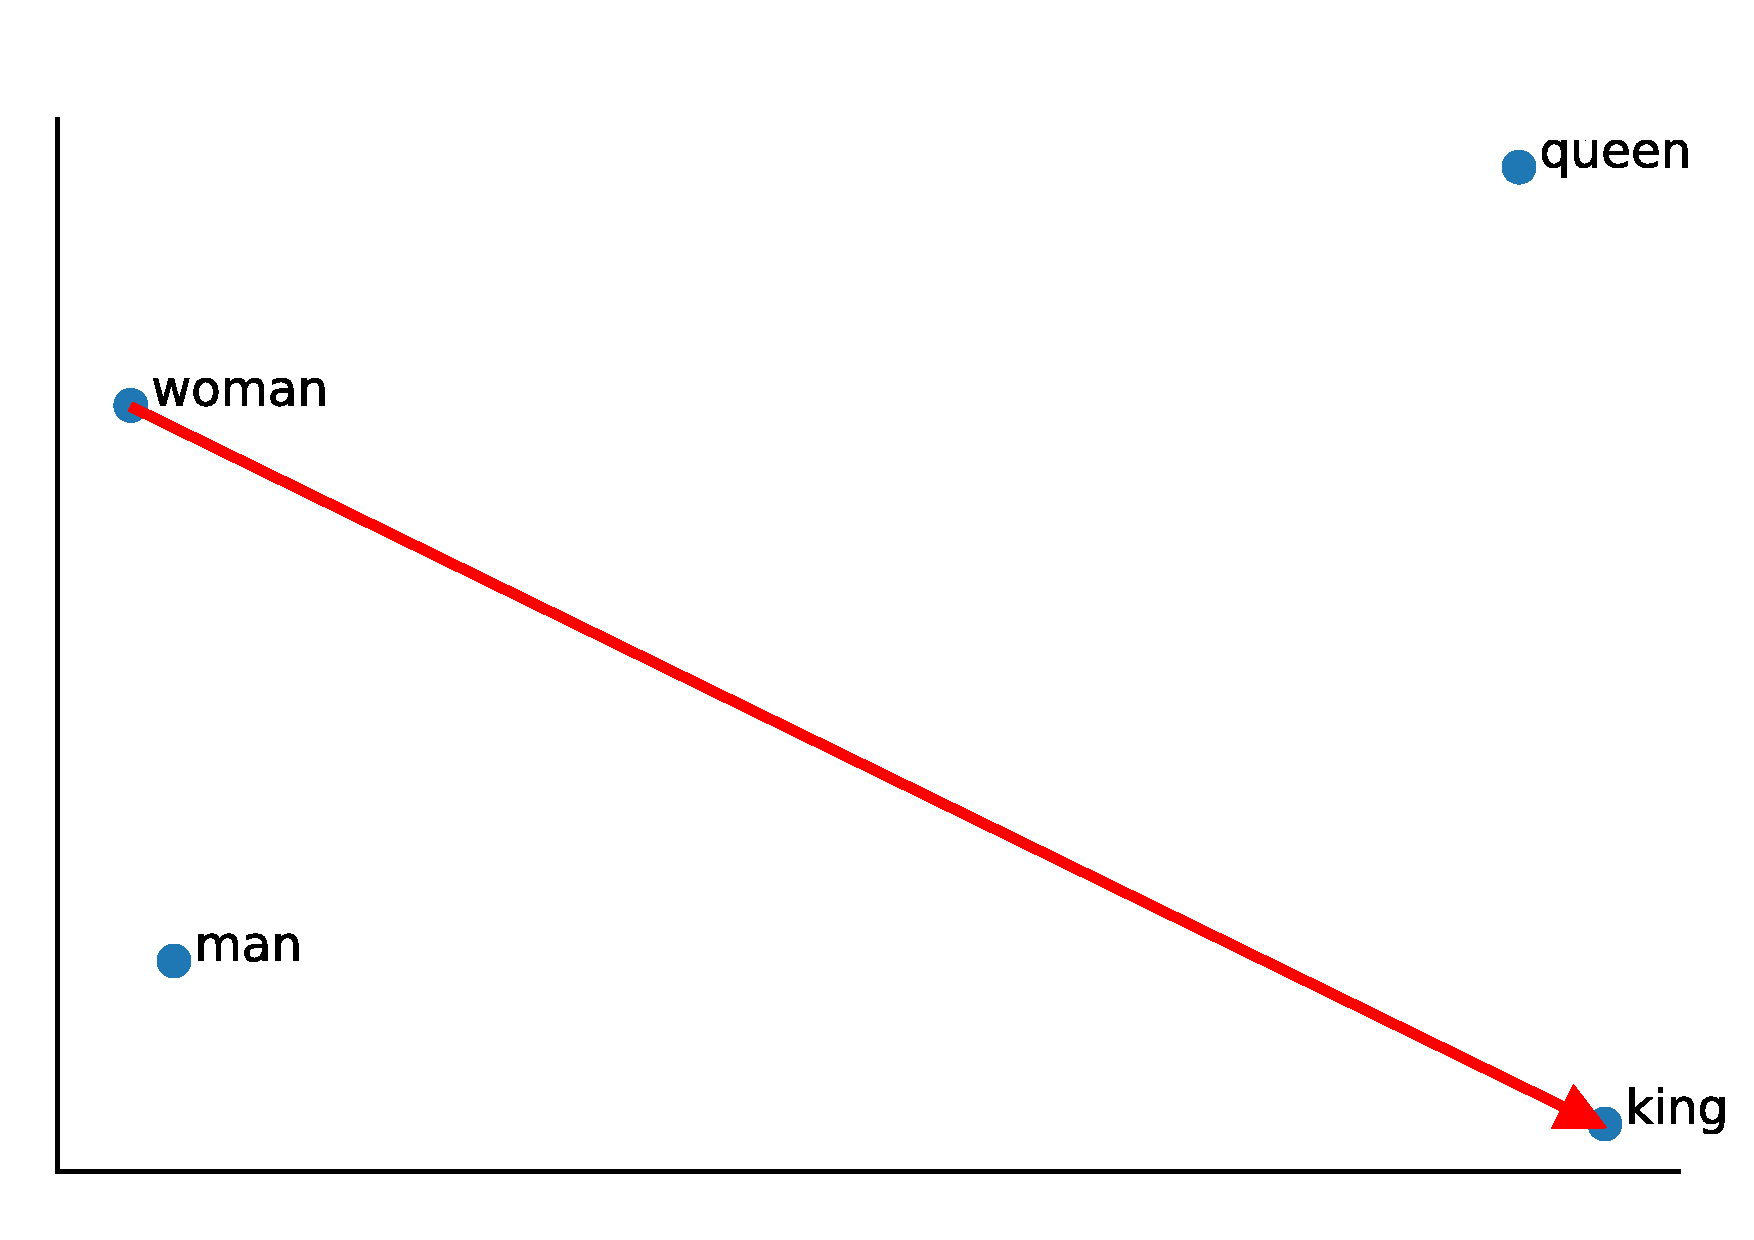
\includegraphics[height=5cm]{Bilder/models/euclidean}
				\caption{Euclidean Distance as Measure}
			\end{minipage}
			\hfill
			\begin{minipage}{0.49\textwidth}
				\label{fig:cosine}
				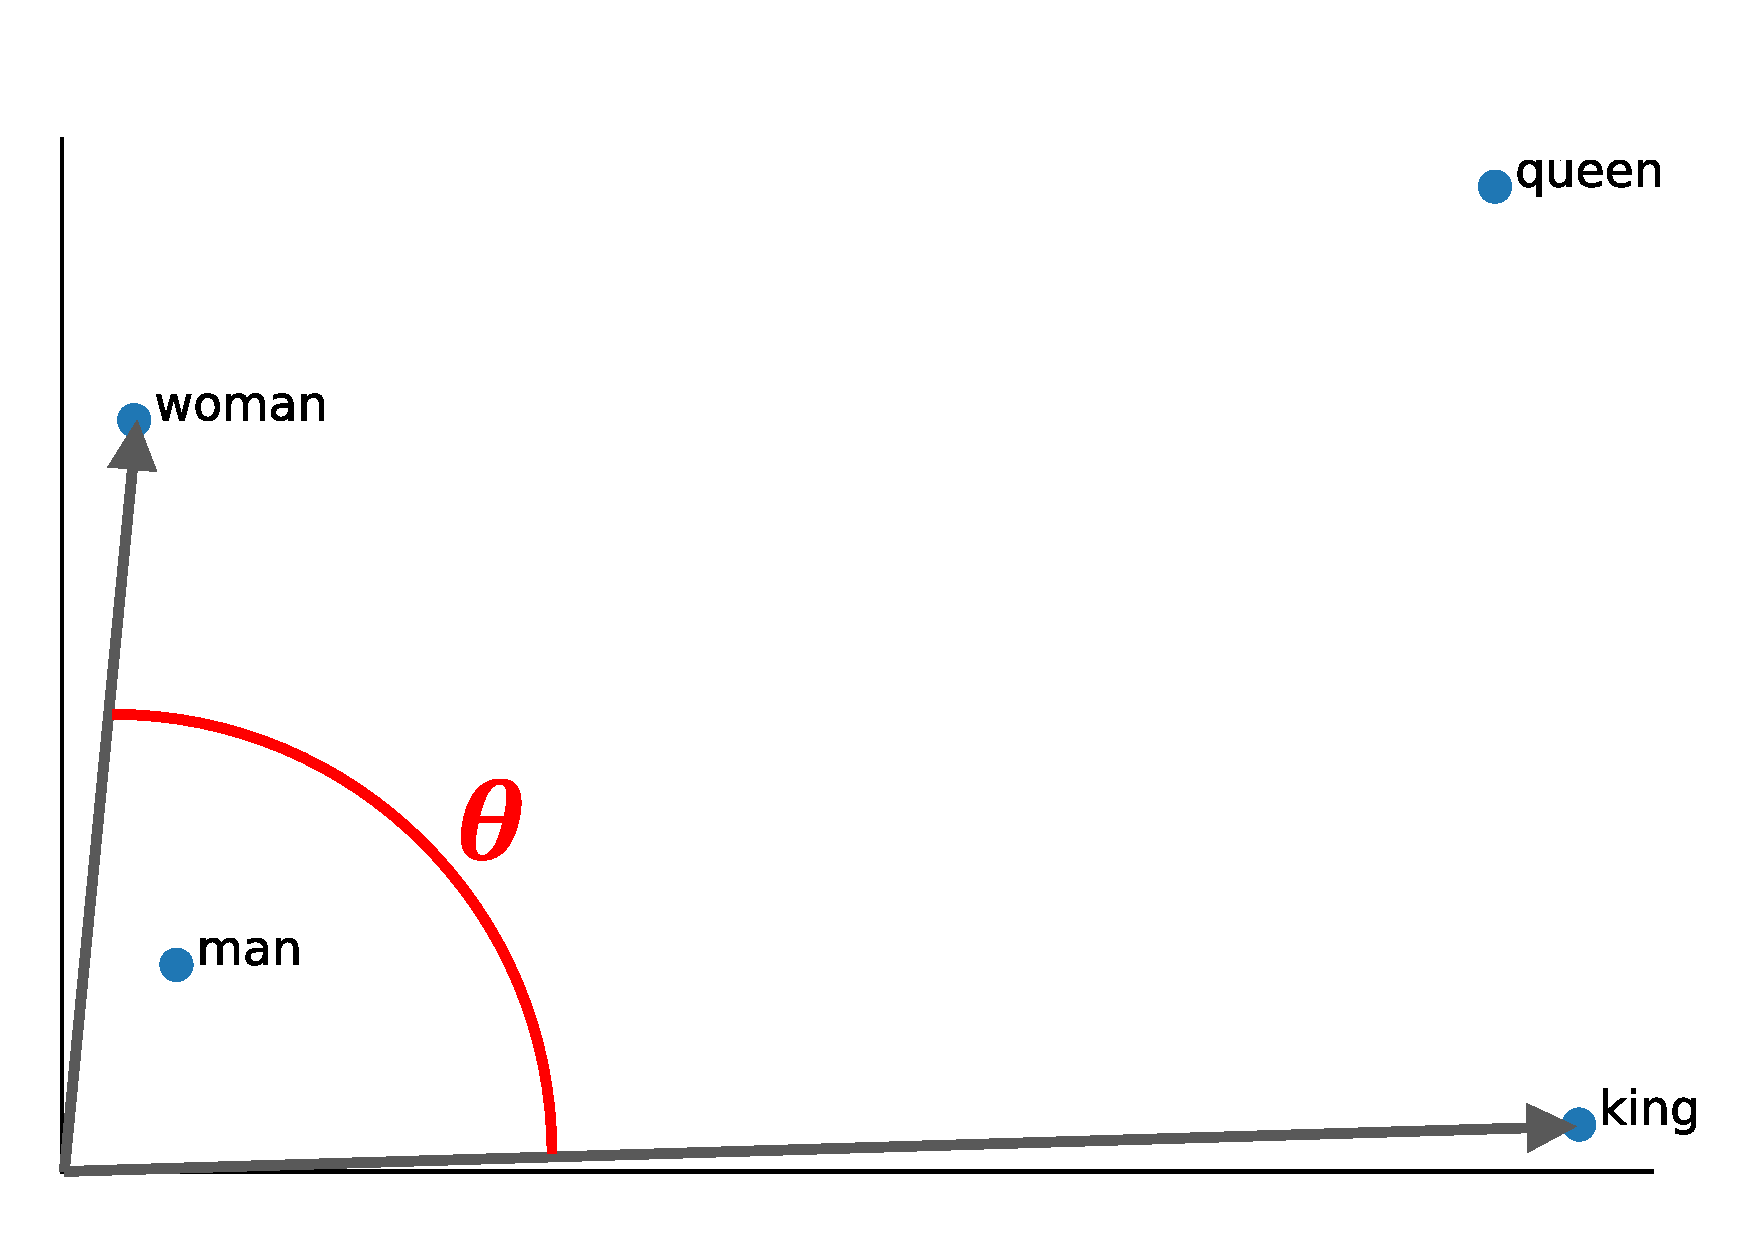
\includegraphics[height=5cm]{Bilder/models/cosine}
				\caption{Cosine Similarity as Measure}
			\end{minipage}
			\hfill
		\end{figure} 
	
		\subparagraph{Cosine Similarity}
		The name of this measure already suggests that not distance but similarity of objects is measured. Instead, it quantifies how close two vectors are. The euclidean distance does not perform well in high-dimensional space, but cosine similarity is highly accurate even for high-dimensional data  \cite{40algorithms}. Mathematically, the cosine distance is the cosine of the angle between two vectors. A wide angle means a high distance between two vectors, or in this case two words. Narrow angles stand for a low distance and words being closely related. In example \ref{fig:cosine}, the word vectors for woman and king have a higher angle than those of woman and queen. This means the words woman and queen are more similar thank woman and king.
		
		\[ 
		\text{cosine similarity} := \cos(\theta) = {\mathbf{A} \cdot \mathbf{B} \over \|\mathbf{A}\| \|\mathbf{B}\|} = \frac{ \sum\limits_{i=1}^{n}{A_i  B_i} }{ \sqrt{\sum\limits_{i=1}^{n}{A_i^2}}  \sqrt{\sum\limits_{i=1}^{n}{B_i^2}} }
		  \]
		
		
\subsection{Clustering Algorithms}
		
		\subparagraph{K-Means}
		The k-Means algorithm generates $k$ groups of data by iteratively adapting clusters and their centers. The algorithm is mainly focused on performance, hence the design is kept lean by omitting logic for determining the number of clusters \cite[c.~6.2]{40algorithms}. Following pseudo code illustrates the workings of the algorithm.
		
		\begin{lstlisting}
randomly choose k_centers
while (iterations < max_iterations):
	assign each point to nearest center in k_centers
	mean of each cluster's elements are k_centers_new
	if k_centers == k_centers_new:
		break
		\end{lstlisting}
	
			 \begin{figure}[!h]
		\centering
		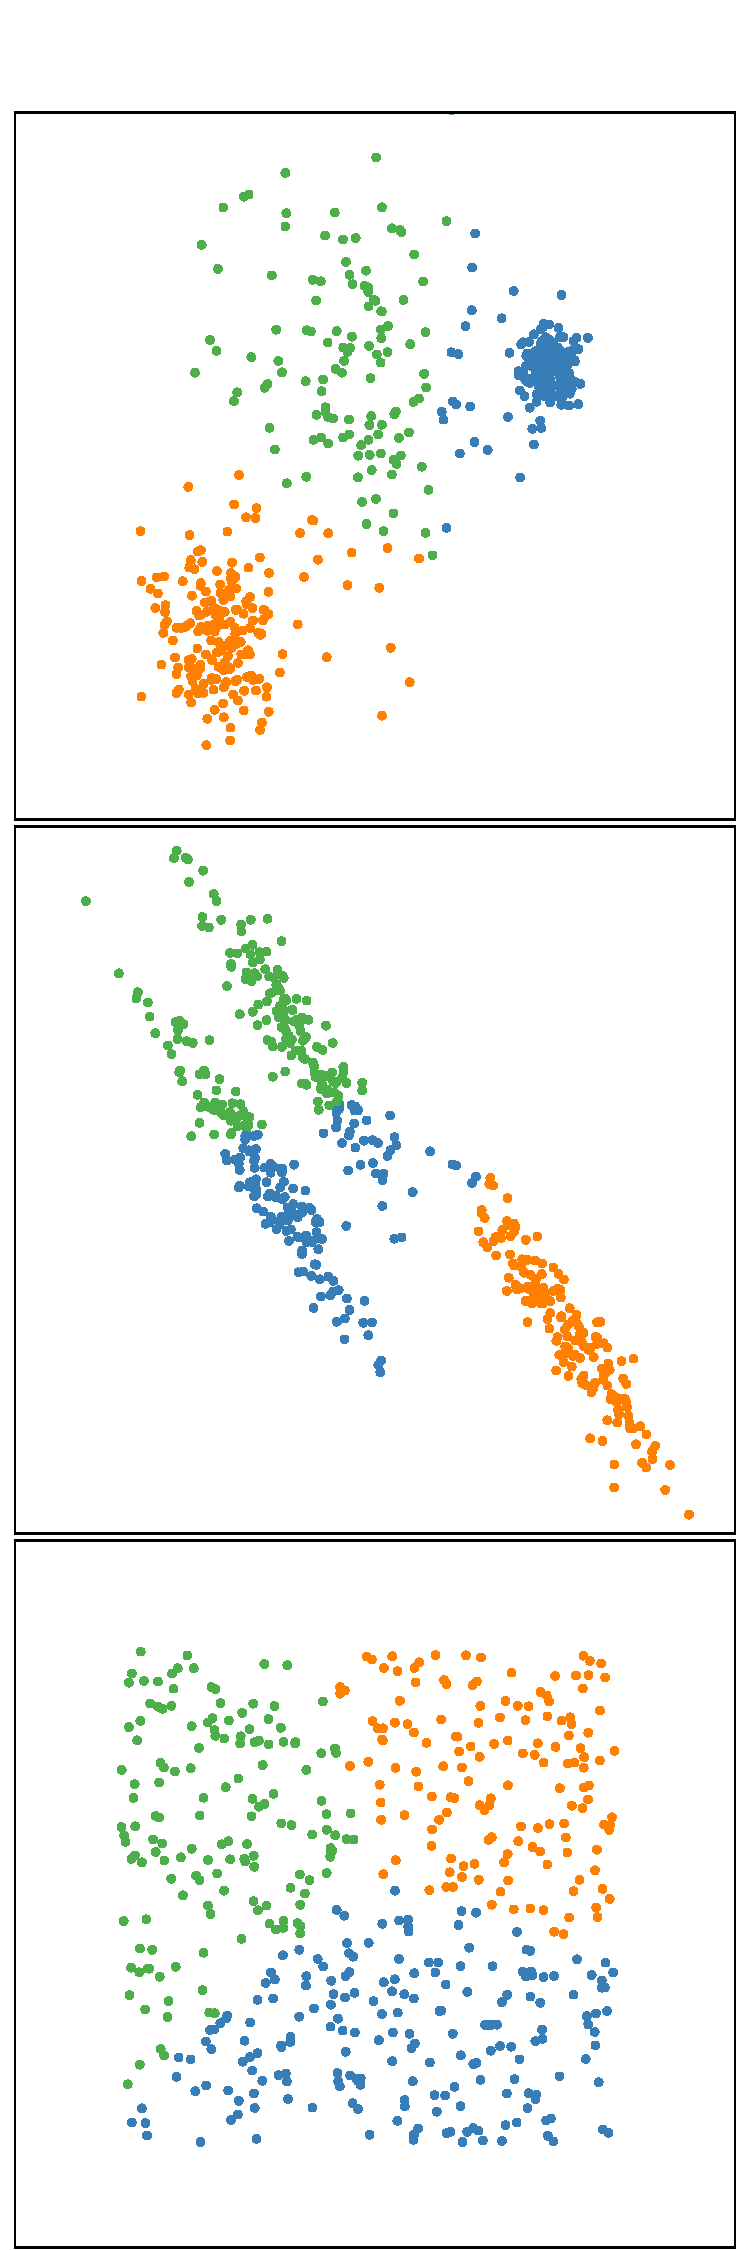
\includegraphics[height=15cm, angle=90]{Bilder/models/minibkmeans.pdf}
		\caption{How MiniBatchKmeans recognizes Clusters \cite{sklearn}}
		\label{fig:kmeans-viz}
		\end{figure}
	
		The k-Means algorithm performs reasonably well in identifying clusters in data such as in figure \ref{fig:kmeans-viz}. The left example seems unspectacular, but in the center example, it becomes obvious that k-Means is prone to overfit on noisy data. This can be partially blamed on the focus on centers, and not density. The focus on centers is also obvious in the rightmost example. While the data is quite evenly distributed over the area, the algorithm still groups the data. 
		
		Implementations such as \ac{sklearn}'s \lstinline|MiniBatchKMeans| \cite{sklearn} speed up the computation time by processing subsets of the data in a parallel way. While only achieving almost perfect results \cite{sculleyWebscaleKmeansClustering2010}, the batched k-Means algorithm is of special appeal when handling large data sets.
		
		This algorithm has the advantage of high performance, and performs well on large data sets. Unfortunately, the quality of the results depend highly on choosing the correct parameters. Also, k-Means is not robust against outliers, and results are not reproducible since the first cluster centers are chosen randomly \cite[c.6.2]{40algorithms}.
		
		\subparagraph{\acl{DBSCAN}}
		The \ac{DBSCAN} clustering algorithm was developed to solve the problem of needing domain knowledge while tuning cluster models \cite{DBSCAN}. The algorithm uses an intuitive approach for identifying which points belong into a cluster, and which are outliers.

		For two points to be considered neighboring (density-reachable, \cite{DBSCAN}), they have to be within a certain distance to each other: \lstinline|eps|. Neighboring points are categorized into one cluster, expanding the reach of this cluster over all values within the distance \lstinline|eps|.
		But, there is a limitation to the points being able to expand a cluster. If the cluster were to expand without limitations apart from a maximum distance, the clusters would be able to "spread" from one cluster to another if connected by one data point.
		To prevent this, only center points can expand the cluster. A center point has a minimum number of neighboring points (\lstinline|min_samples|). This helps to create dense clusters and prevents the undesirable spreading.
		
		 \begin{figure}[!h]
			\centering
			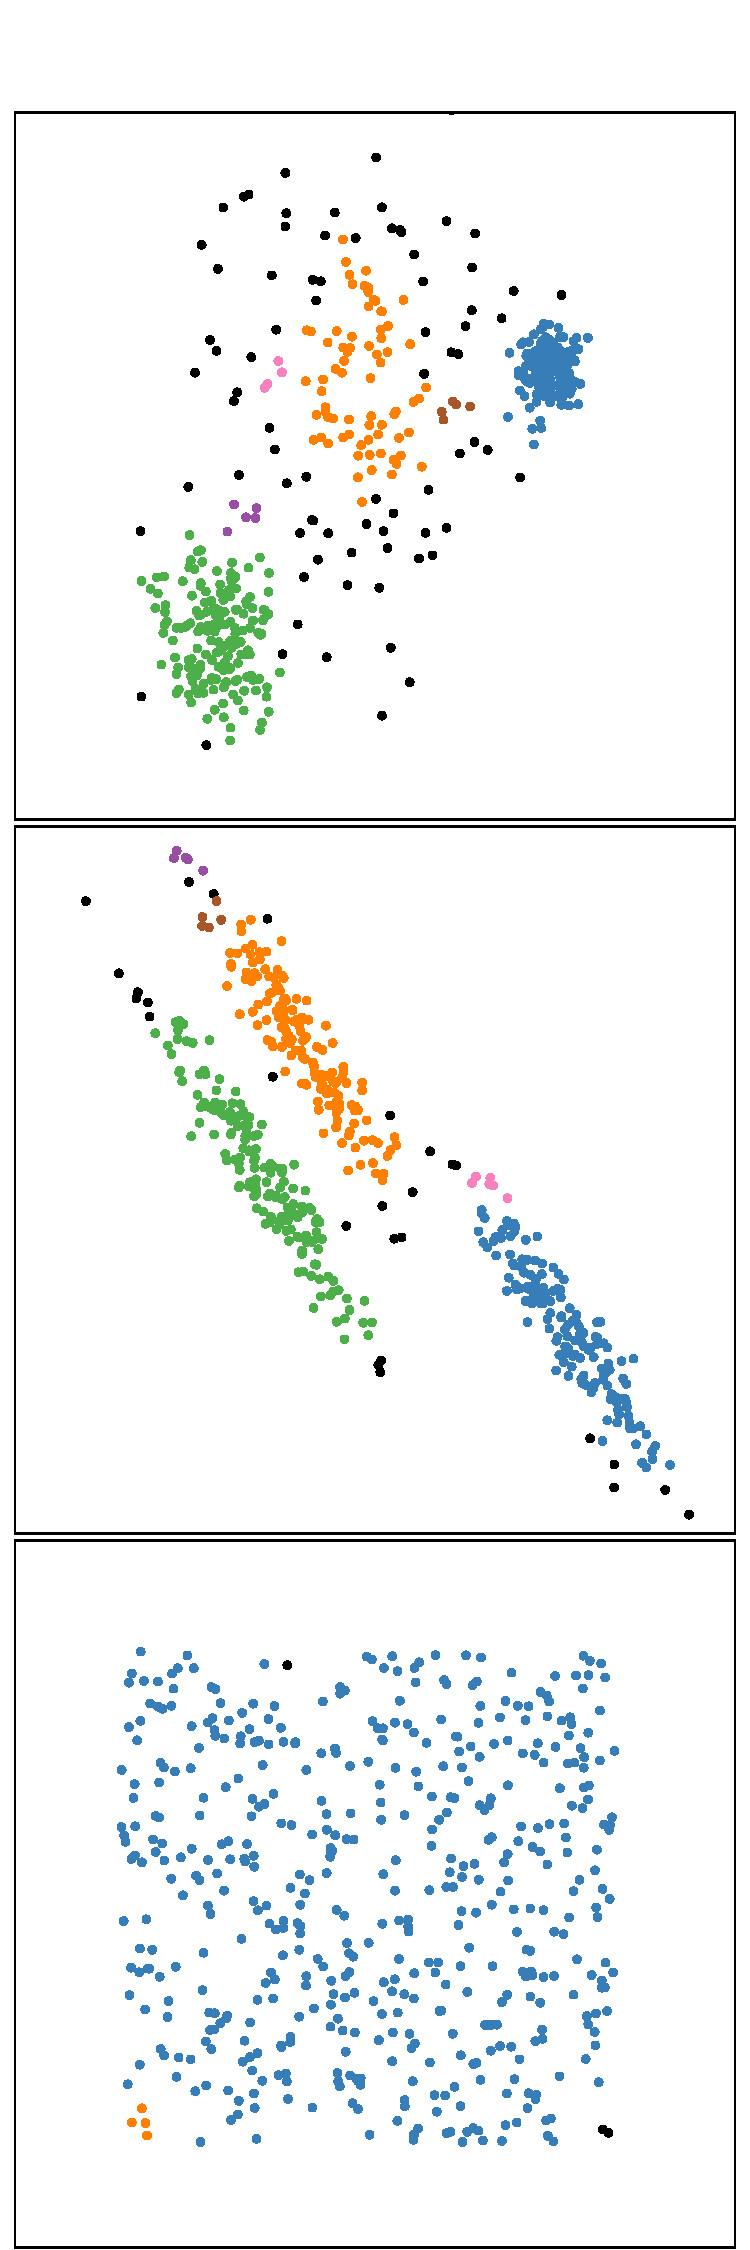
\includegraphics[height=15cm, angle=90]{Bilder/models/dbscan.pdf}
			\caption{How DBSCAN recognized Clusters and Outliers \cite{sklearn}}
			\label{fig:dbscan-viz}
		\end{figure}
	
		Figure \ref{fig:dbscan-viz} illustrates how \ac{DBSCAN} does not fall prey to outliers, as k-Means does. A broad distribution of data points in the left example is very intuitively grouped into clusters and outliers. Especially the center picture showcases the ability of DBSCAN to recognize clusters by their density. The even spread of data in the third example is also correctly identfied as one large cluster, even though a small part of the data was not within \lstinline|eps| range.
		
		

		
\subsection{Topic Model}
After documents are clustered, each cluster needs a meaningful label to provide actual value. This task is called topic modeling. Several methods exist for generating or extracting labels from clustered data. 

Firstly, the word frequency in one cluster can determine the topic. Each word is evaluated with respect to its frequency over the whole cluster. Either the most frequent one or top n words can be the topic.
This method is quite prone to skewing by one document containing a word many times.

The second method uses the document frequency. This measure is also part of the \ac{TF-IDF} measure (\ref{section:tfidf}).
The \ac{TF-IDF} vectorization method had to basic assumptions:
\begin{enumerate}
	\item Words with a high frequency in a document describe it well.
	\item Words with a high frequency in a corpus do not describe one specific document well.
\end{enumerate}

But the second assumption does not hold true any more when applied to a cluster. Clusters should already be very similar, and contain similar words. Therefore, words occurring often over many different documents describe the cluster very well. The metric for this is the document frequency:

\[ DF(t_{i}) =\dfrac{\#(d_{t_{i}}) }{|C|} = \dfrac{ number \; of \; documents \; containing \; word \; t_{i}}{number \;  of\;  documents \;  in \; cluster \; C} \]

The document frequency of a word is the relative share of documents in the cluster it occurs in.

\subsection{Dimensionality Reduction}

The embeddings generated in the data preparation section are 512-dimensional. While the clustering algorithms work well with processing this data, 512 dimensions are not imaginable with the human mind. To visualize clusters, these dimensions have to be projected onto a two-dimensional plane. This task is called \ac{DR}, and is unsupervised. 

Selecting a \ac{DR} method, there are important aspects to consider:
\begin{itemize}
	\item How well can the algorithm preserve the distances in the clusters (local structure)?
	\item How well can the algorithm preserve the distances between the clusters (global structure)?
\end{itemize}

Data scientists have many methods for \ac{DR} at hand, some of the most popular ones being \ac{t-SNE} and \ac{PCA}.

The \ac{PCA} identifies principal components in the dataset with an unsupervised \ac{ML} algorithm.\cite{40algorithms} A principal component is an axis in the multidimensional space along which the variance is maximized \cite{pcaVStsne}. The number of learned principal components depends on the number of target dimensions, in the case of visualizations either two or three dimensions and principal components. The principal components are orthogonal to each other and span the hyperplane on which the values are projected \cite{pcaVStsne}.
It is important to note that \ac{PCA} approximates the values, trading in accuracy for performance \cite{40algorithms}.

\ac{t-SNE} is focused on retaining as much structure, both globally and locally. It does so by computing pairwise similarities in the dataset. The algorithm uses these similarities to accurately represent the same distances in a lower number of dimensions. This design of \ac{t-SNE} helps to represent existing clusters very well.

The two methods are contrasted on the task of representing three-dimensional clusters (Figure \ref{original}) in two dimensions. This task is quite similar to the later application of the \ac{DR} algorithm. In figure \ref{fig:pca} the \ac{PCA} algorithm proves that it is able to represent the global structure in some way, but not quite satisfactory. It is heavily outperformed by \ac{t-SNE}, in both preserving the global distances and the local structures. Apart from two clusters merging, the algorithm forms very distinct and clean clusters.

Overall, design and the practical application of the \ac{t-SNE} algorithm make the case for it.

\begin{figure} 
	\begin{minipage}{0.3\textwidth}
		\label{fig:origina}
		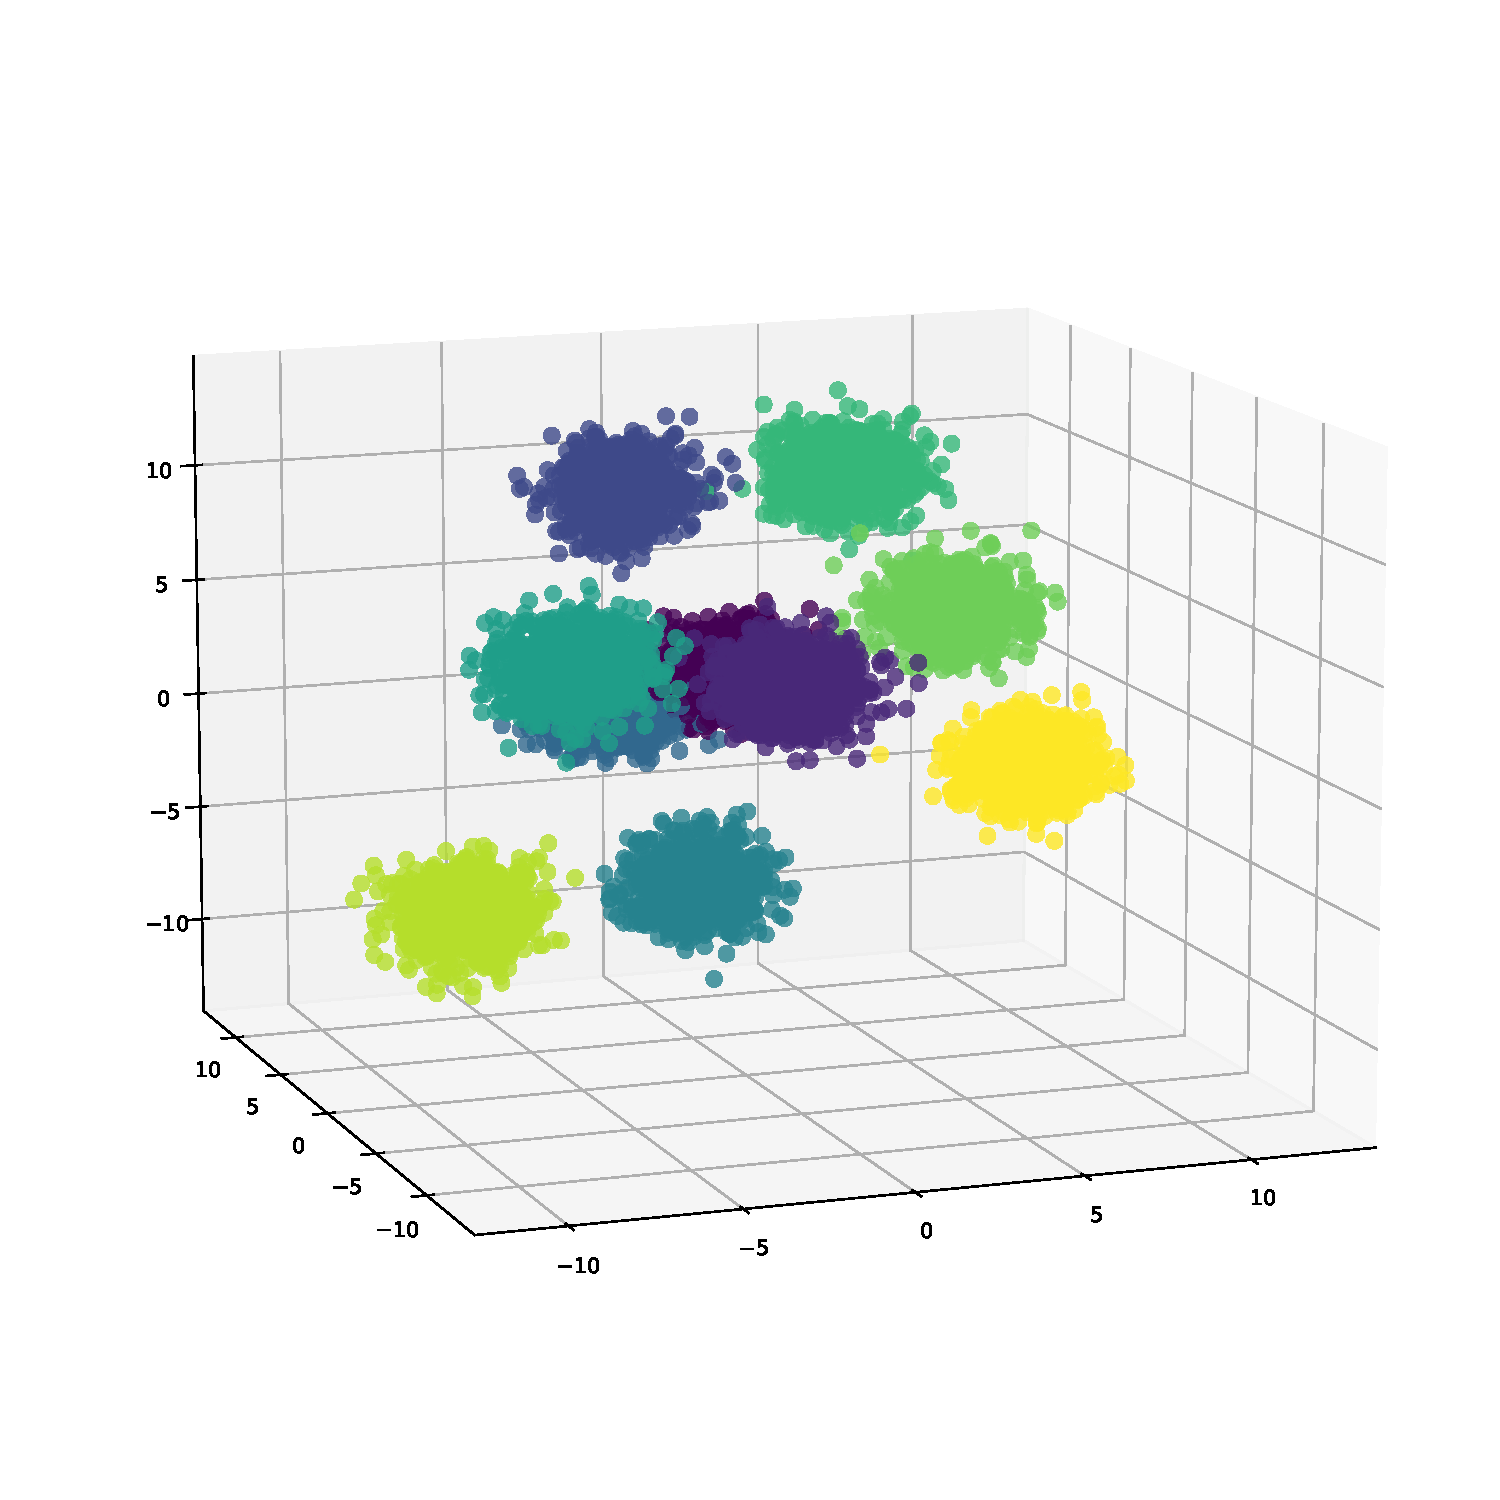
\includegraphics[height=5cm]{Bilder/models/original.pdf}
		\caption{Three-dimensional Clusters}
	\end{minipage}
	\hfill
	\begin{minipage}{0.3\textwidth}
		\label{fig:pca}
		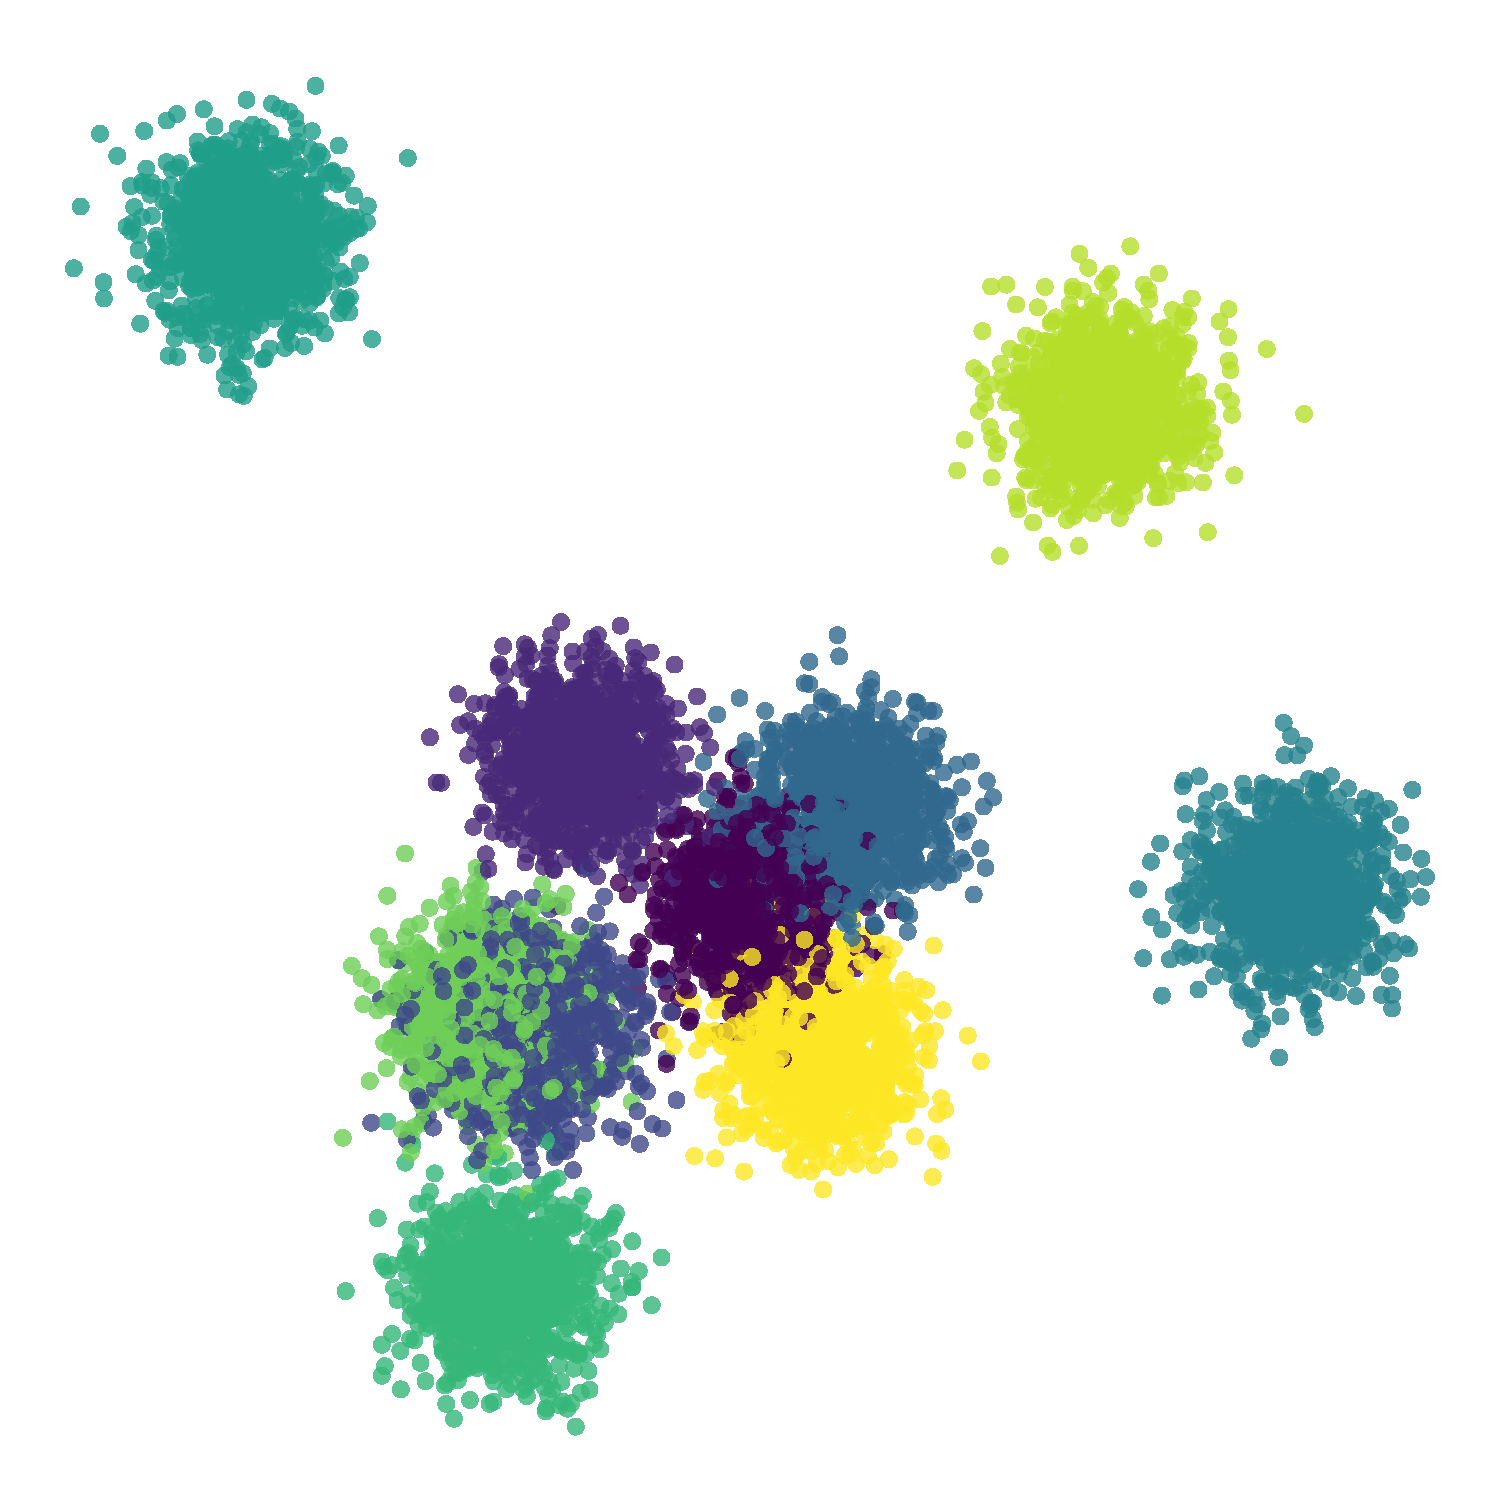
\includegraphics[height=4cm]{Bilder/models/pca.pdf}
		\caption{\ac{PCA}}
	\end{minipage}
	\hfill
	\begin{minipage}{0.3\textwidth}
		\label{fig:tsne}
		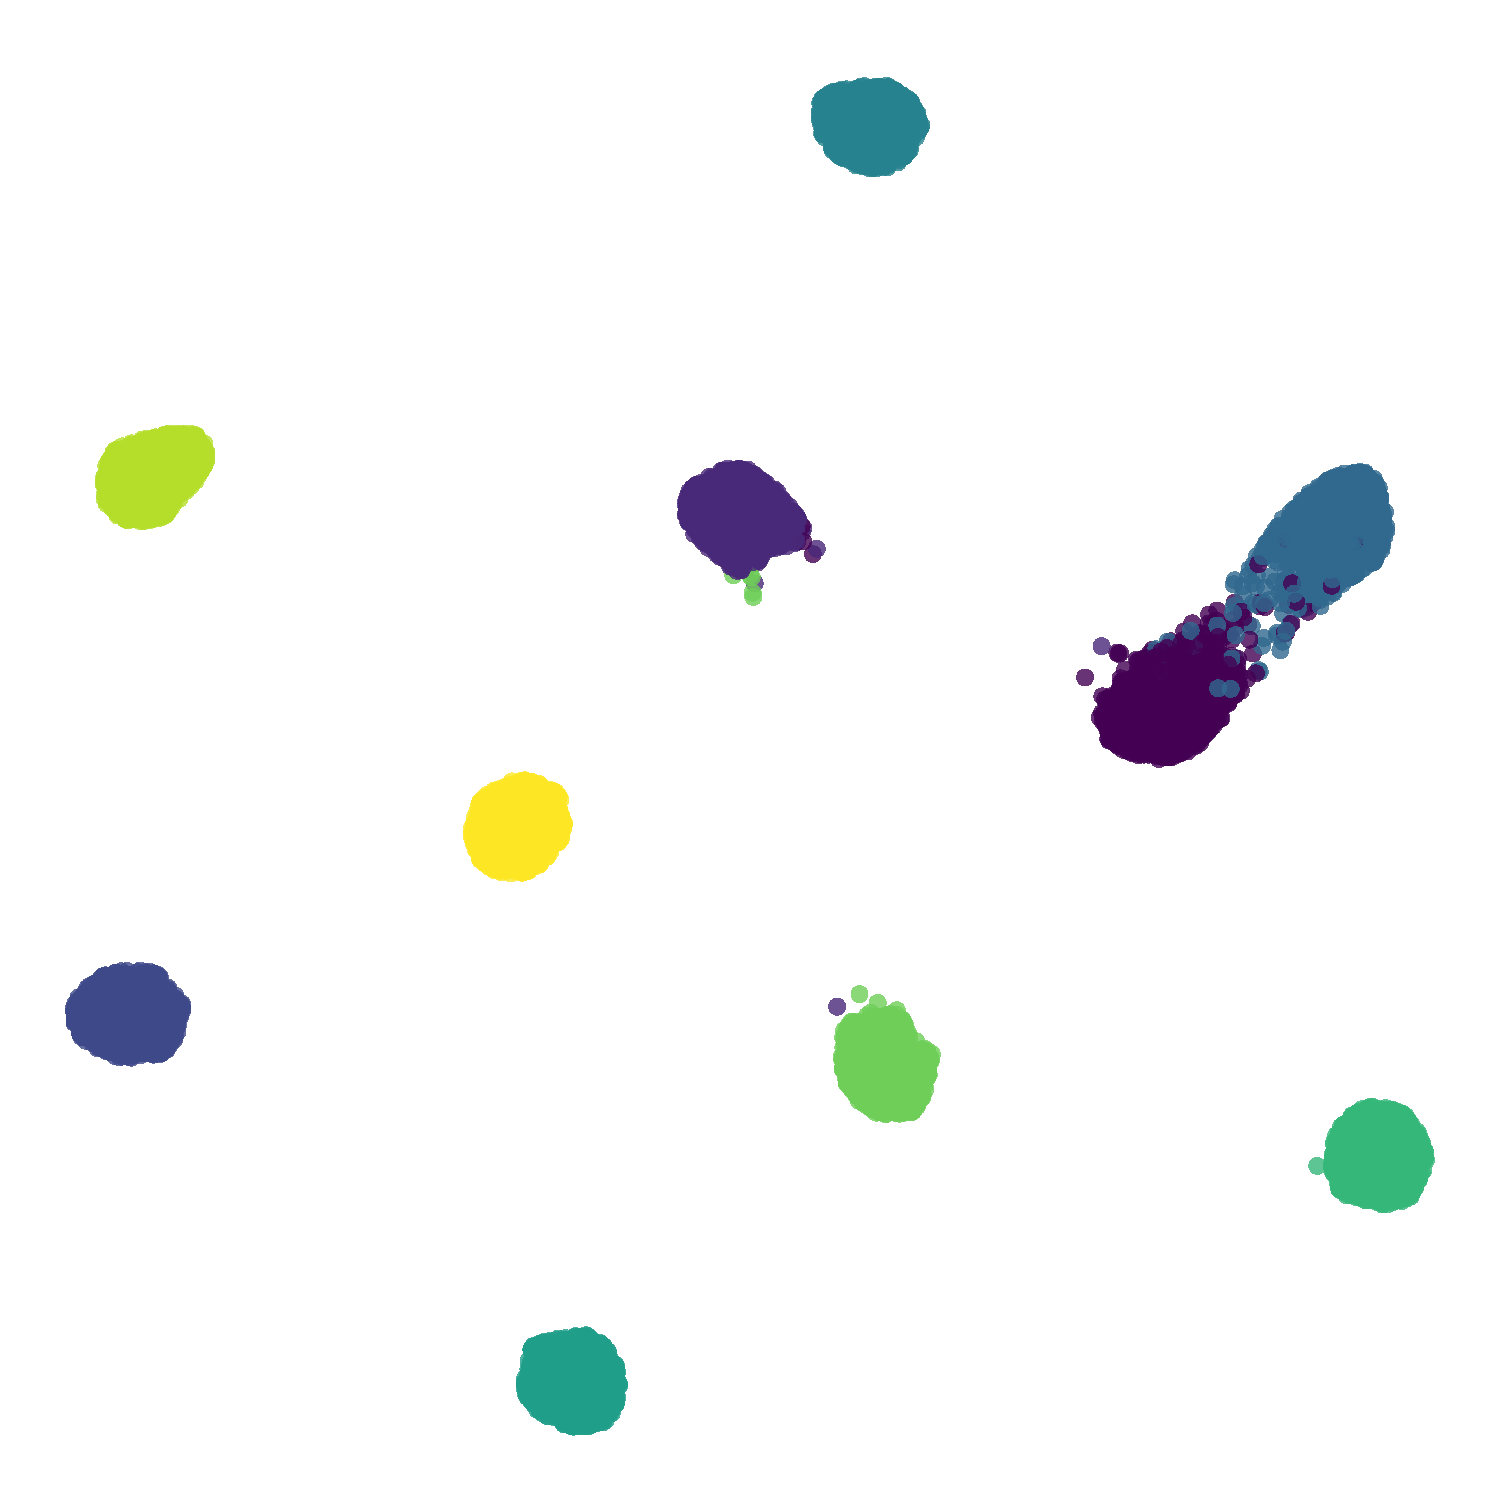
\includegraphics[height=3.5cm]{Bilder/models/tsne.pdf}
		\caption{\ac{t-SNE}}
	\end{minipage}
\end{figure} 

\section{Theoretical Implementation}

\begin{table}[]
	\label{table:modeling}
	\begin{tabular}{lll}
		\textbf{Task}            & \textbf{Alternatives}                                                                      & \textbf{Planned Implementation}                                                               \\
		Distance Measure         & \begin{tabular}[c]{@{}l@{}}Dot Product\\ Euclidean Distance\\ Cosine Distance\end{tabular} & Cosine Distance                                                                               \\
		Clustering               & \begin{tabular}[c]{@{}l@{}}k-Means\\ DBSCAN\end{tabular}                                   & \begin{tabular}[c]{@{}l@{}}DBSCAN for outlier detection\\ k-Means for clustering\end{tabular} \\
		Topic Modeling           & \begin{tabular}[c]{@{}l@{}}Word Frequency\\ Document Frequency\end{tabular}                & Document Frequency                                                                            \\
		Dimensionality Reduction & \begin{tabular}[c]{@{}l@{}}PCA\\ t-SNE\end{tabular}                                        & t-SNE                                                                                        
	\end{tabular}
\end{table}


The table \ref{table:modeling} sums up all available alternatives from the prior section and the chosen alternative. The implementation of the modeling part starts with an analysis of the cosine distances in the dataset. For this, the KNeighbors algorithm will show the distance of each datapoint to its next neighbor. Next the outliers are sorted out with the DBSCAN clustering method. Before training the k-Means model, the ideal number of clusters has to be found with the elbow method. The k-Means model identifies the clusters. Topics per cluster are generated and the clusters are visualized with t-SNE.



\section{Practical Implementation}

\subsection{Determining composition of dataset with KNeighbors Algorithm}


Both density-based and distance-based clustering algorithms work with distances between objects. Before any clustering is applied, an overview over the distances should be established \cite{maklinDBSCANPythonExample2022a}. This allows to make meaningful decisions while hyperparameter-tuning.

 \begin{figure}[!h]
	\centering
	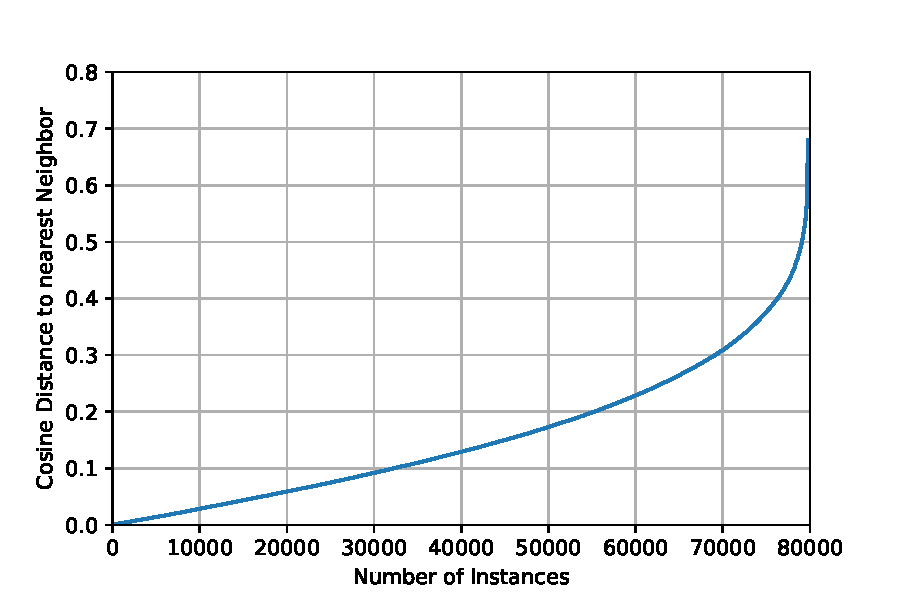
\includegraphics[height=8cm]{Bilder/models/kneighbors.pdf}
	\caption{Each Instance's Distance to the nearest neighboring Point}
	\label{fig:dbscan-plot}
\end{figure}

This can be done with the algorithm \lstinline|sklearn.neighbors.NearestNeighbors|, which takes the input of a dataset with arbitrary dimensions. Using a specified distance metric, the algorithm outputs the distance of each data point to its nearest neighbor in the data set. The distance metric used is the cosine distance.
The distance search shows that almost all points are within a maximum distance of 0.4 to the next neighbor. All other points are outliers and will be filtered out with \ac{DBSCAN}.



\subsection{Preselect documents with \ac{DBSCAN} and cosine distance}
The \ac{DBSCAN} algorithm outputs, apart from clusters, outlier data points which do not belong into any cluster. With this algorithm, outliers in the data are detected to prevent the main clustering algorithm (KMeans) from overfitting. 
The clustering algorithm has the parameters \lstinline|eps| and \lstinline|metric| which tune the model.

The (distance) \lstinline|metric| is of course cosine. The \lstinline|eps| stands for the maximal distance between two points to be considered a neighbor \cite{SklearnClusterDBSCAN}. As established before, the outliers are those points which are more than 0.4 units separated from the next data point. Therefore, \lstinline|eps| is set to 0.4. 

The \ac{DBSCAN} model identified the outlier data (\ref{fig:dbscan-outliers}), amounting to about 3\% of the data points. These data points are not included into clustering by k-Means.

\subsection{Determine the number of clusters with the Elbow Method}
The KMeans algorithm is parameterized with the number of clusters (\lstinline|n_clusters|). Since the algorithm itself is not able to determine the cluster count, this number has to be approximated.
\cite{kodinariyaReviewDeterminingCluster2013} suggest several applicable methods, among them are rule of thumb, and the elbow method with a silhouette score.
A good point for starting with choosing \lstinline|k| is the rule of thumb $k \approx \sqrt{\frac{n}{2}}$ with n being the number of instances in the dataset. Other literature also names the approximation of $k \approx log(n)$, but \cite{maierOptimalConstructionKnearest2009} showcase how $k$ should be chosen in the order of $n$. 

\begin{table}[!h]
	\centering
	
	\begin{tabular}{l|ll}
		\toprule
		heuristic for best k                         & k &  \\
		\midrule
		$k \approx \sqrt{\frac{n}{2}}$ &  199 &  \\
		$k \approx log(n)$             & 12   &  \\
		$k \approx n$                  &  e.g. 10 000, 20 000& 
	\end{tabular}
\caption{Three possible estimates for the optimal $k$}
\label{table:heuristic-k}
\end{table}

With the elbow method, the silhouette score of clustering results for different values of \lstinline|k| are visualized. 

The silhouette score is a measure of how similar intra-cluster points are and at the same time how dissimilar inter-cluster points are. A silhouette score of 1, being the highest value, is the most desirable.

The silhouette score $s$ of each data point $i$ can be calculated with the following formula \cite{kodinariyaReviewDeterminingCluster2013}:
\[ s(i) = \frac{b(i) - a(i)}{\max\{a(i),b(i)\}} \]

The measure $a$ denotes the mean distance to other points in the same cluster as $i$. This is interpreted as the inter-cluster dissimilarity, the higher $a(i)$, the more $i$ doesn't belong into the cluster.

The measure $b$ stands for the mean distance between $i$ and the points in the nearest other cluster. To identify the nearest other cluster to the point $i$, all mean distances to points of each cluster are calculated. The cluster with the smallest mean distance between all its points and $i$ is the neighboring cluster. The measure $b$ is interpreted as the similarity of $i$ to other clusters.

Being calculated for every point, this measure always falls in the interval $[-1;1]$. For $S = 1$, the relationship of $a(i)$ and $b(i)$ has to be $a(i) \ll b(i)$ so that the denominator and divisor each tend to $b(i)$ resulting in $S = 1$. This would mean that the point $i$ would have to be very far away from points in other clusters and very near to its own cluster. The value $S = 1$ is therefore the most desirable.

For $S = 1$, the relationship of $a(i)$ and $b(i)$ has to be $a(i) \gg b(i)$ so that the denominator and divisor each tend to $-a(i)$ respective $a(i)$ resulting in $S = -1$. In distance terms this means that the point $i$ is very far away from its own cluster points and very close to points in the next nearest cluster.

Therefore, the task of the elbow method using the silhouette coefficient is to maximize $S$ while preventing overfitting.

The above mentioned estimates (\ref{table:heuristic-k}) are a starting point for choosing values for k during the calculation of silhouette coefficients.


\subsection{Train a KMeans Model}

\subsection{Visualize cluster formation}
\subsection{Generate Topics per cluster with \ac{LDA}}



		
\include{Inhalt/04_Inhalt/content_evaluation}
\chapter{Deployment}

Tableau Dashboard

%\chapter{Discussion of Alternatives}
\section{Criteria}
\section{KMeans}
\section{Deep Learning}
\section{Data Cleaning}
\section{Tf-Idf}
\section{K-Means}
\subsection{Elbow Diagram}
\subsection{Visualizations}
\section{Embeddings}
\section{Transformers}
\section{Dimensionality Reduction}
%\chapter{Theoretical Implementation}

%\chapter{Practical Implementation}

\section{Dataset selection}
	T
	
\section{Data preparation}


	\subsection{Data processing and data wrangling}
	
	The data for an invoice and its contained items is stored in an array of objects. This is also shown in code example (\ref{code:JSONSchema}) of a shortened JSON Schema for one invoice. The array "annotations" contains objects. One object represents information such as the invoice date or the unit price. 
	Information about invoice items have labels containing the prefix "lineItem". One invoice containing several items is represented by duplicate values of one label (in the example \ref{code:JSONInvoice} the label "lineItem.description.value"). Here, the order of the labels has to be retained during data wrangling to ensure not mixing up information about different invoice items.

	\lstinputlisting[
	label=code:JSONInvoice,    % Label; genutzt für Referenzen auf dieses Code-Beispiel
	caption=JSON of one invoice,
	captionpos=b,               % Position, an der die Caption angezeigt wird t(op) oder b(ottom)
	style=EigenerPythonStyle,   % Eigener Style der vor dem Dokument festgelegt wurde
	firstline=0,                % Zeilennummer im Dokument welche als erste angezeigt wird
	lastline=23                 % Letzte Zeile welche ins LaTeX Dokument übernommen wird
	]{Quellcode/invoice.json}
	
	The files are processed in python, using the library "json". Each file is opened, and decoded with python's build in json decoder. The hierarchy is traversed until the array "annotations" is reached. Now, the tuples of label and text are saved. This process is split up into invoice and item labels.
	
	The information on invoices is stored in a tabular data structure, a python pandas DataFrame. Worth mentioning is that some invoices contain more information than others. In this case, invoices are still appended into one table, but fields for non-existent values are left empty. The filename is the unique identificator for one invoice.
	
	\begin{figure}[ht]
		\centering
		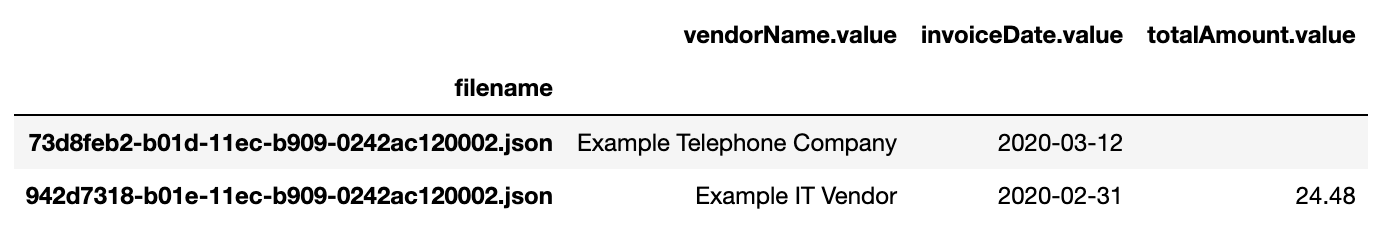
\includegraphics[height=2.5cm]{Bilder/practical/df_invoices.png}
		\caption{Exemplary depiction for processed invoices in a DataFrame}
		\label{fig:df-invoices}
	\end{figure}

	Similarly, information on the invoice items is retrieved from the documents and stored in a pandas DataFrame. Every invoice item has an unique id and can be linked to the respective invoice through the filename.
	
	\begin{figure}[ht]
		\centering
		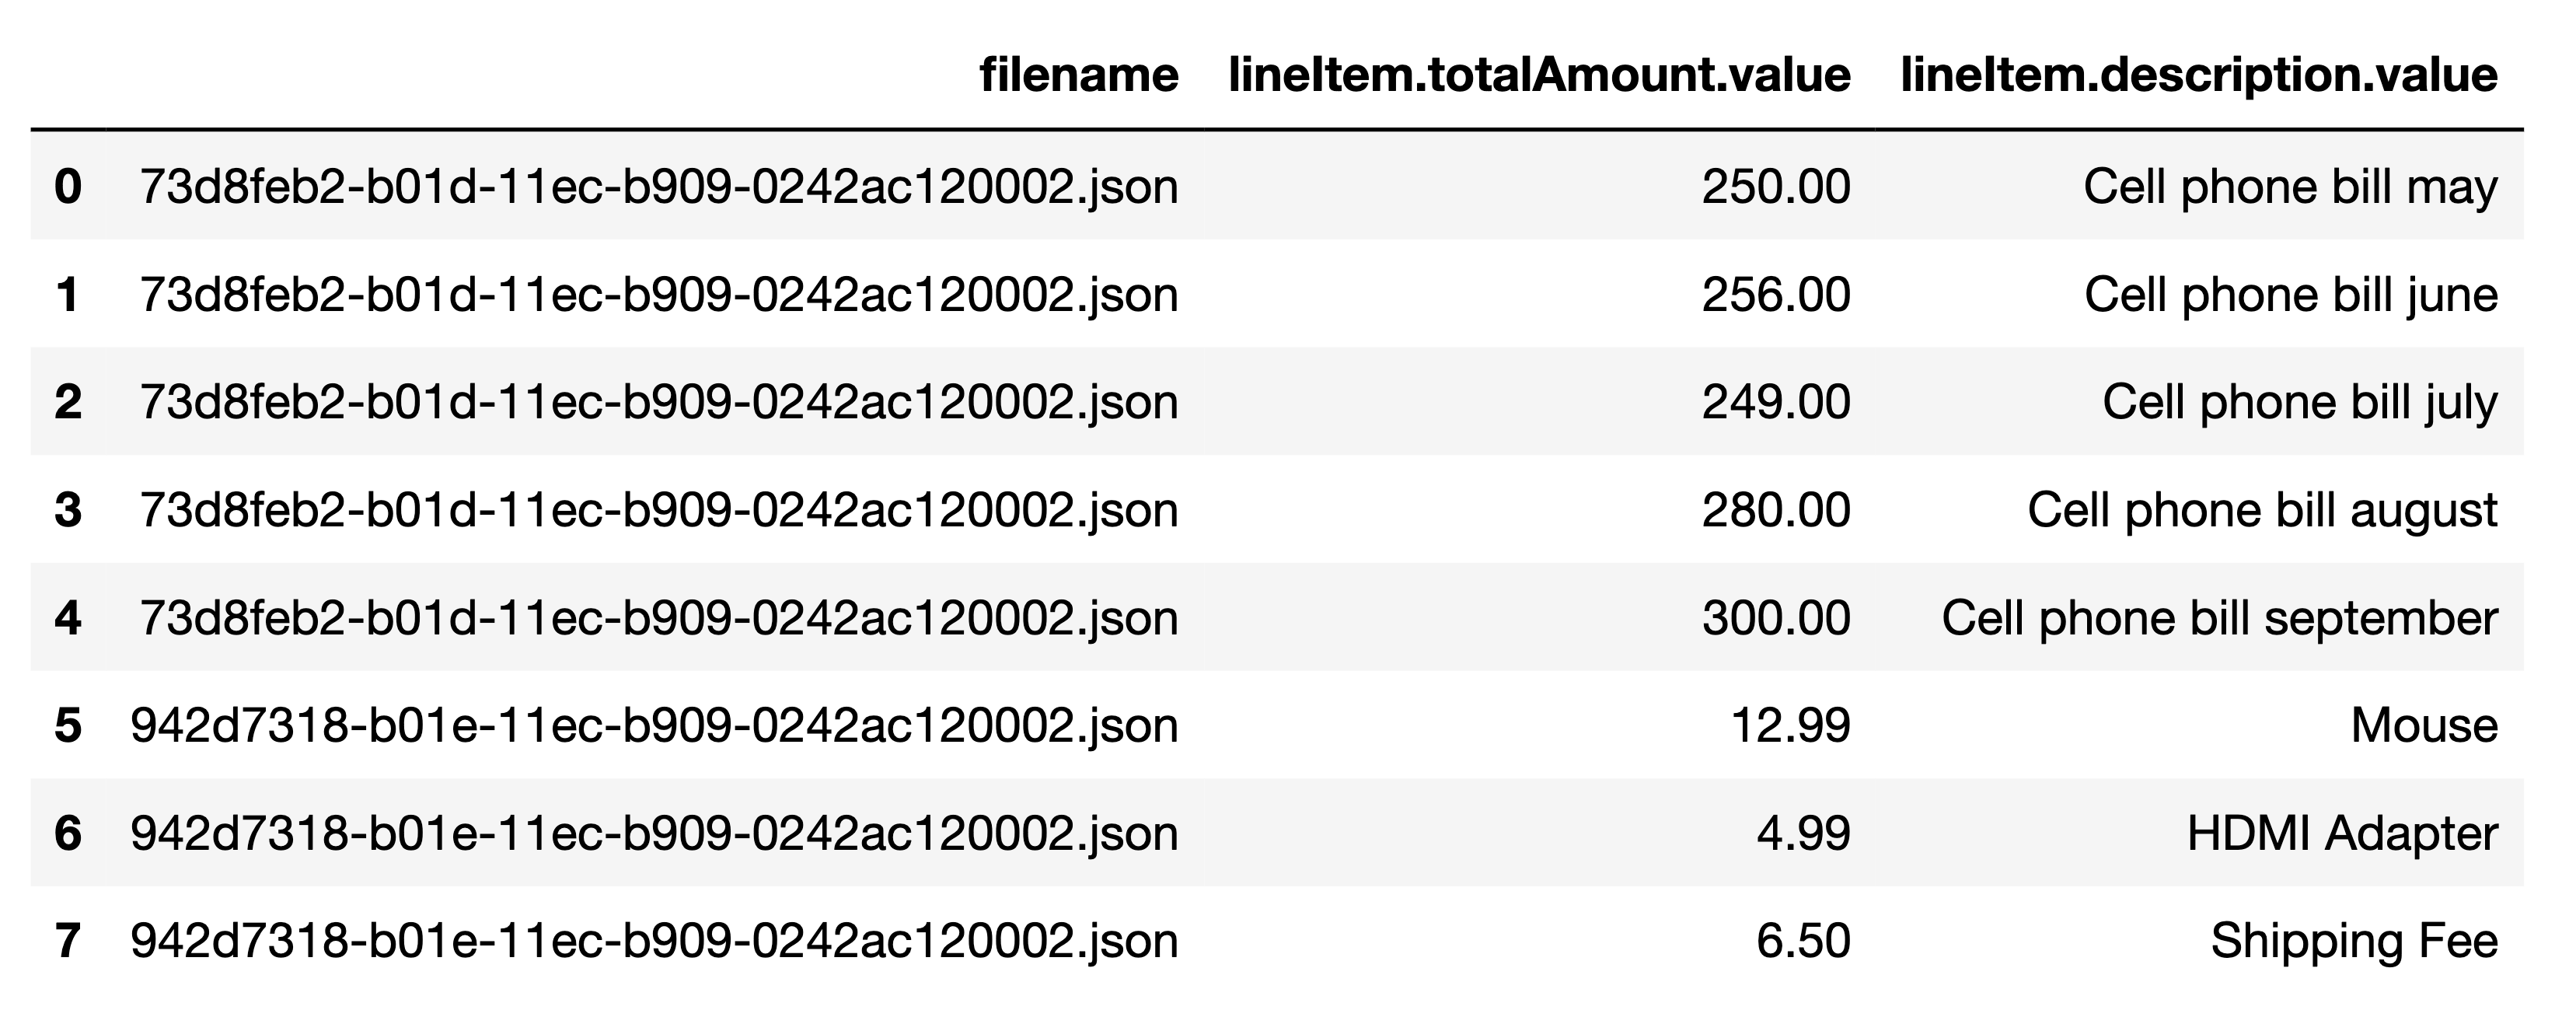
\includegraphics[height=6cm]{Bilder/practical/df_lineitems.png}
		\caption{Exemplary depiction for processed invoice items in a DataFrame}
		\label{fig:df-invoices}
	\end{figure}
	
	The resulting two DataFrames are serialized with the python standard library "pickle".  The data can be efficiently loaded into memory and reserialized again with this library.
	
	This processing step allowed for storing the initial 5.12GB of data in a more usable format and takes up only a total of 393MB. Even further improvements to storage will be dicussed later on.

	The process of reading files from the disk is not inherently an expensive one, but in the realms of many thousand documents, processing times soon reach several days. Observing the execution of the python code showed a peculiarity: While the utilization of the used processor was consequently at the maximum, only one process is executed, leaving the total CPU usage at only 20\%. 
	
	\begin{figure}[ht]
		\centering
		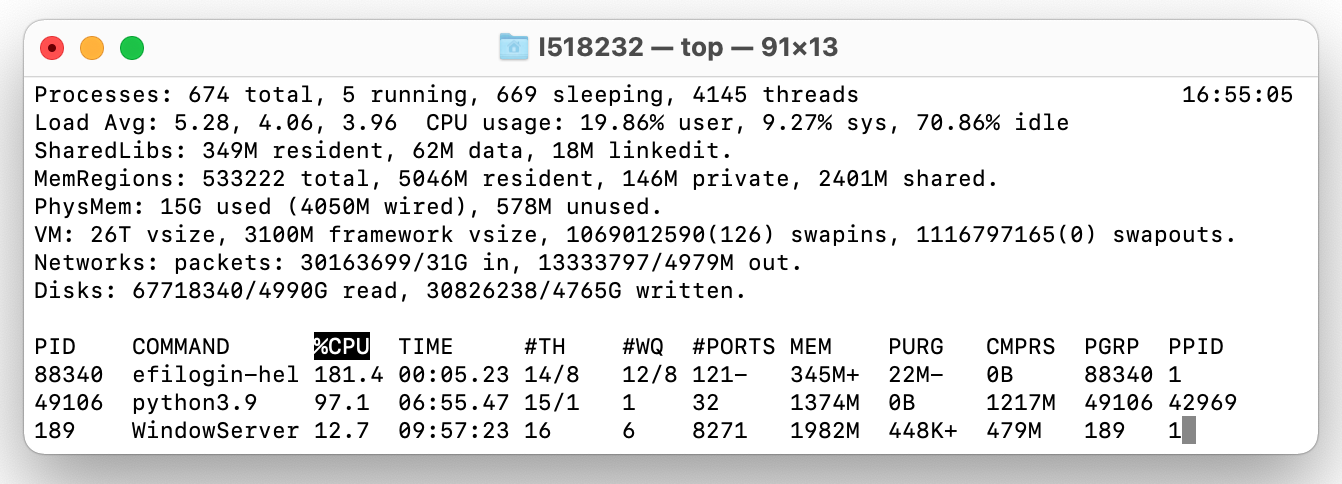
\includegraphics[height=4cm]{Bilder/practical/python_processes.png}
		\caption{Exemplary depiction for processed invoice items in a DataFrame}
		\label{fig:df-invoices}
	\end{figure}
	
	
	One question that may now arise is: Why doesn't python split up the workload and employ the full capacity of the machine?
	This can be explained with the design of the Python interpreter. The \ac{GIL} controls access to the Python Virtual Machine executing the code. This lock only allows exactly one thread to run at a time \cite{corePython}. This of course is not favorable, as valuable CPU capacity is unused. Fortunately, the \ac{GIL} behaves in a special way regarding C code, and I/O operations in Python utilize C code: the lock is released before executing a C routine \cite{corePython}. This allows to bypass the (in this case) inconvenient locking mechanism. 
	
	Different python libraries exploit this speciality and allow to spawn a pool of different processes, which then execute calls asynchronously. One example is the ProcessPoolExecutor. A notable restriction is that only picklable objects can be submitted for multiprocessing. This concerns both fuction and its parameters. While this is not a problem in this task, this restriction will become important later on in the section about feature extraction.
	
	\lstinputlisting[
	label=code:JSONSchema,    % Label; genutzt für Referenzen auf dieses Code-Beispiel
	caption=Shortened JSON Schema of one invoice document representation,
	captionpos=b,               % Position, an der die Caption angezeigt wird t(op) oder b(ottom)
	style=EigenerPythonStyle,   % Eigener Style der vor dem Dokument festgelegt wurde
	firstline=0,                % Zeilennummer im Dokument welche als erste angezeigt wird
	lastline=23                 % Letzte Zeile welche ins LaTeX Dokument übernommen wird
	]{Quellcode/json-schema.json}
	
	

	
	\subsection{Data cleaning}
	
	\subsection{Considerations of Space and Time Complexity}
	The dataset consists of over 150.000 invoices, and in those invoices, over 350.000 items are listed. 
	With hardware-limitation in place, an optimized approach for storing and processing the data is required. 
	Several considerations for speeding up processing time and reducing storage space can be made. 
	In the following, the observations are explained and approaches for improvement are given.

		\subsubsection{Duplicates and space complexity}
		Investigation shows, there are only 79.741 unique descriptions for the listed items. By saving only the unique values, the required space is reduced to less than one fourth compared to before. Additionally, this step is required by most machine learning models, as duplicate input values can skew the outcome. The model is chosen later, so this processing step leaves the model selection more open to different kinds of learning algorithms.
		
		\subsubsection{Reconstructing Relationships and time complexity of searching}
		After the deletion of duplicate descriptions (documents in the corpus), the 
		
		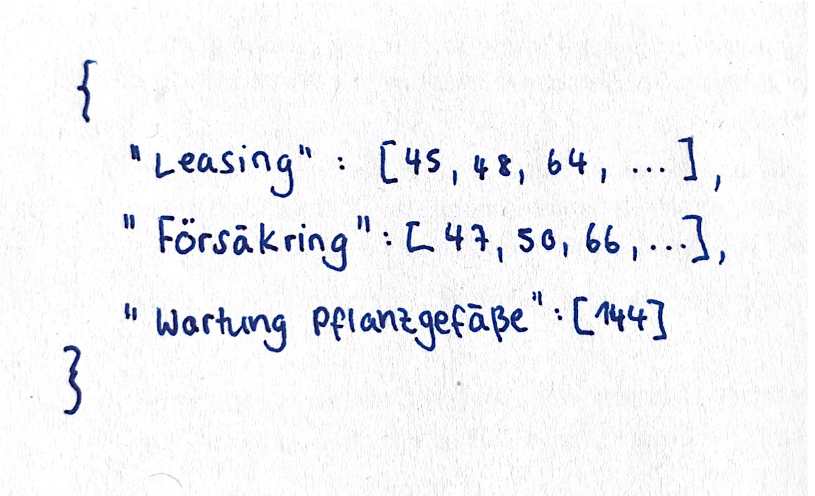
\includegraphics[height=8cm]{Bilder/description_map.png}

	\subsection{Feature Extraction and Feature Engineering}

\section{Modelling}
\section{Evaluation}
	\subsection{Visualization}
\section{Deployment}

\chapter{Evaluation of the result}
\section{Visualization}
\section{Measures}
\include{Inhalt/04_Inhalt/Outlook}
% ---- Literaturverzeichnis
\cleardoublepage
\renewcommand*{\chapterpagestyle}{plain}
\pagestyle{plain}
\pagenumbering{Roman}                   % Römische Seitenzahlen
\setcounter{page}{\numexpr\value{savepage}+1}
\printbibliography[title=References]

% ---- Anhang
\appendix
%\clearpage
%\pagenumbering{Roman}  % römische Seitenzahlen für Anhang
\chapter{Appendix}
\begin{table}[]
    \caption{Inventory of Resources}
    \begin{tabular}{lll}
    \textbf{Type of resources} & \textbf{Kind of resources} & \textbf{Quantification}                                                    \\
    Personnel                  & business experts           & 1 person                                                                   \\
                               & data experts               & 1 person                                                                   \\
                               & technical support          & 1 person                                                                   \\
                               & data mining experts        & 1 person                                                                   \\
    Data                       & fixed extracts             & -                                                                \\
                               & live data                  & -                                                                          \\
                               & warehoused data            & -                                                                          \\
                               & operational data           & 1 dataset                                                                         \\
    Computing resources        & hardware platforms         & \begin{tabular}[c]{@{}l@{}}1 machine \\ access to SAP AI Core\end{tabular} \\
    Software                   & data mining tools          & anaconda, jupyter                                                          \\
                               & other relevant software    & Excel, Visual Studio Code, Git                                                                     
    \end{tabular}
    \label{tabelle:inventory}
    
    *) An asterisk indicates theoretical availability of more resources, if needed.
    \end{table}

\newpage
\end{document}
